\clearpage
\setcounter{page}{1}
\setcounter{section}{0}
\setcounter{figure}{0}
\setcounter{table}{0}
\maketitlesupplementary
\renewcommand\thesection{\Alph{section}}
\renewcommand{\thetable}{S\arabic{table}}    % 修改表格标签
\renewcommand{\thefigure}{S\arabic{figure}}  % 修改图片标签

\section{Overview}
\vspace{-1mm}
This supplementary material provides additional details on dataset construction, implementation, and extended experiments supporting the main paper. The sections are organized as follows:
\begin{itemize}
    \item \textbf{\cref{sec:models}}: Model configurations of G-Tok, the autoregressive generator, and the multimodal style encoder.
    \item \textbf{\cref{sec:data_dist}}: Data curation and partitioning, covering both training and evaluation protocols.
    \item \textbf{\cref{sec:quant_ext}}: Extended quantitative results, including scaling analyses of our autoregressive generator.
    \item \textbf{\cref{sec:Ablate}}: Detailed and visualized ablations of key design choices in GAR-Font.
    \item \textbf{\cref{sec:vis_results}}: Extensive qualitative results for visual-only and multimodal FFG, along with error analyses.
    \item \textbf{\cref{sec:Failure_cases}}: Analysis of GAR-Font failure cases in dense-stroke and complex font styles.

    
\end{itemize}

%%%%%%%%%%%%%%%%%%%%%%%%%
\section{Model Configuration}
\label{sec:models}
Table~\ref{tab:model-structure} details the architectural specifications of GAR-Font. The framework relies on three core components: (1) The \textbf{Global-aware Tokenizer (G-Tok)} , which employs a hybrid CNN-ViT architecture to discretize glyphs into a compact codebook ($N=2048$); (2) The \textbf{Autoregressive Generator}, which serves as the synthesis backbone, using a deep Transformer decoder to predict tokens conditioned on aggregated content and style features; and (3) The \textbf{Multimodal Style Encoder}, which utilizes a lightweight adapter to align textual embeddings with visual style representations for text-driven control.
\begin{table}[h]
\centering
\small
\setlength{\tabcolsep}{3pt} % 调小列间距
\begin{tabular}{p{0.8\columnwidth} c}
\toprule
\textbf{Key Components} & \textbf{Params (M)} \\
\midrule
\textbf{G-Tok} & 79.59 \\
CNN Encoder & 28.56 \\
ViT Encoder (layers = 6) & 4.73 \\
Codebook (size = 2048, dim = 8) & 0.02 \\
ViT Decoder (layers = 6) & 4.73 \\
CNN Decoder & 41.42 \\
\midrule
\textbf{AR-Generator} &  346.23 \\
Content Encoder & 28.56 \\
Visual Style Encoder & 2.78 \\
Content-style Aggregator (layers = 3) & 0.79 \\
Transformer Decoder (layers = 24) & 314.10 \\
\midrule
\textbf{Multimodal Style Encoder} & 8.04 \\
Projection & 0.52 \\
Visual Style Encoder & 2.78 \\
Language-Style Adapter (layers = 6) & 4.74 \\
\bottomrule
\end{tabular}
\vspace{-3mm}
\caption{Key GAR-Font components and parameter counts.}
\vspace{-3mm}
\label{tab:model-structure}
\end{table}
\begin{figure}[t]
  \centering
  % You will insert the python-generated PDF here
  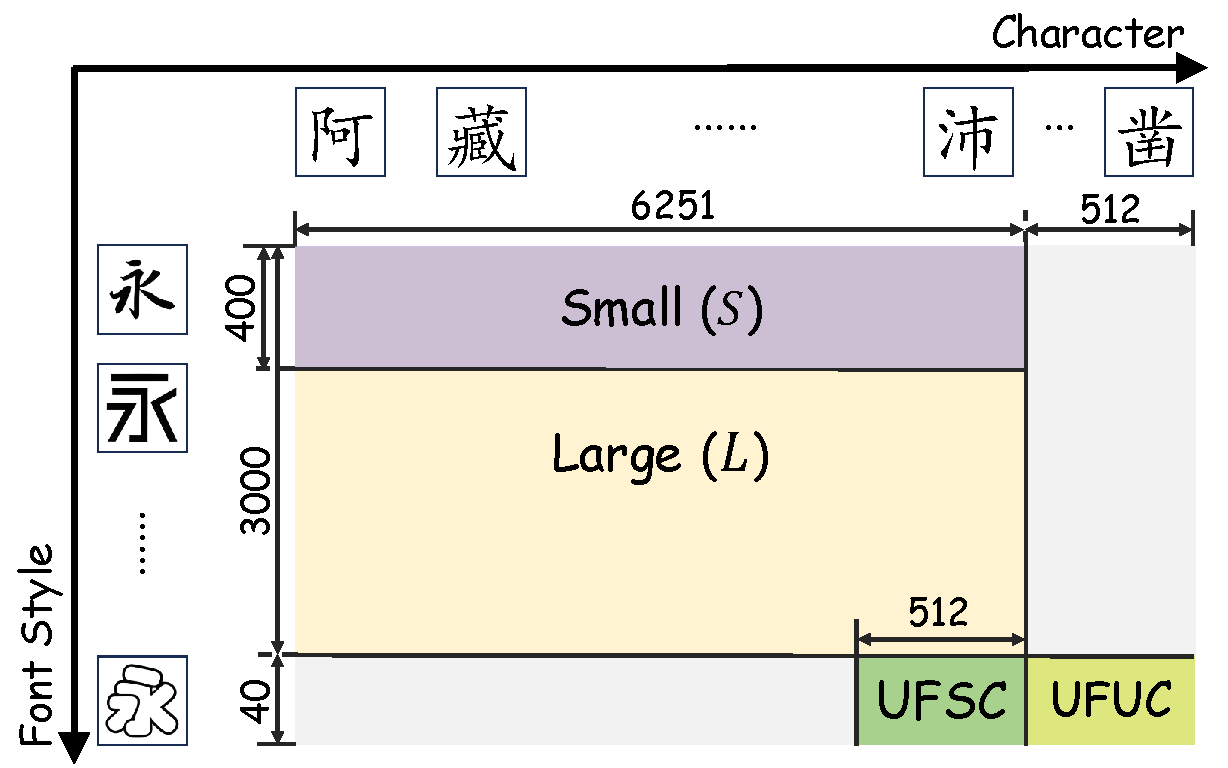
\includegraphics[width=0.95\linewidth]{SUPP_IMGS/data_visualization.pdf} 
  \vspace{-3mm}
  \caption{\textbf{Visual illustration of the dataset partition.} The data is organized along font and character axes. Pre-training utilizes the purple and yellow regions ($S$ and $L$). Evaluation is conducted on the bottom green regions (\textit{UFSC} and \textit{UFUC}), strictly isolating unseen styles and characters.}
  \vspace{-3mm}
  \label{fig:data_viz}
\end{figure}


\section{Data Curation}
\label{sec:data_dist}

\subsection{Data Collection and Statistics}
\label{ssec:data_stats}
We construct a comprehensive font dataset derived from the official GB2312 character set. As illustrated in \cref{fig:data_viz}, the whole training and test dataset is structured as a matrix spanned by two orthogonal axes: \textit{Font Style} (vertical axis) and \textit{Character Category} (horizontal axis). 
The collected data comprises 3,040 fonts and 6,763 characters. 

For training data, along the Character Axis, we split 6,251 training characters (left column) and left 512 characters unseen (right column). The unseen characters are reserved strictly for testing to evaluate the model's capability to generate novel glyph structures. Similarly, the font library is divided into 3,000 training fonts (top rows) and 40 unseen test fonts (bottom rows).


\subsection{Pretraining Data}
\label{ssec:data_pretrain}
The pretraining phase utilizes the data located in the upper-left quadrant of \cref{fig:data_viz}, defined by the intersection of training fonts and training characters. Within this quadrant, we define two configurations to investigate scaling behaviors:
\begin{itemize}[leftmargin=*]
    \item Large ($L$): The full training block consisting of all 3,000 training fonts paired with the 6,251 training characters (represented by the blue region).
    \item Small ($S$): A subset consisting of the first 400 training fonts paired with the same 6,251 characters (represented by the reddish overlay).
\end{itemize}
Training on $S$ versus $L$ allows us to assess the model's data efficiency and performance scaling with respect to the diversity of source styles.

\subsection{Textual Prompt Collection}
\label{ssec:prompt}

To support multimodal few-shot font generation (FFG), we construct a consistent textual prompt set that captures font-level stylistic attributes. For each font, we randomly sample 40 glyph images and jointly input them into Qwen-VL 2.5. The model is instructed to produce a single, unified description summarizing only the visual properties that remain consistent across the full glyph set—such as stroke weight, curvature, structural proportions, spatial rhythm, edge texture, and overall tonal characteristics. This process yields a controlled and stylistically coherent textual representation for each font.

The exact prompt used for textual description extraction is provided below:

\begin{FontExtractPrompt}
You are an experienced typographic style analyst. You are given a set of glyph images belonging to the same font. Your task is to synthesize a unified stylistic description that captures only the consistent, font-level visual attributes shared across the full glyph set.

Your output must adhere to the following specifications:

\textbf{1. Required Format}  

Provide a single paragraph that:

- begins with the phrase “A font that …”,

- contains approximately 45–50 words,

- includes only stylistic properties observable across all glyphs,

- avoids speculative or uncertain expressions.

\textbf{2. Allowed Stylistic Dimensions}  

Constrain your analysis to the following attributes:

- stroke weight (light, medium, bold, uniform, contrasting),

- curvature (straight, angular, rounded, flowing, sharp),

- structural proportions (compact, tall, wide, balanced),

- spacing and rhythm (tight, loose, even, irregular),

- edge rendering (smooth, sharp, rough, brush-like),

- overall tone or mood (elegant, modern, classical, playful, gentle, formal).

\textbf{3. Constraints}  

All statements must be visually grounded in the provided glyph set. Do not reference features specific to individual characters. The description must reflect global stylistic coherence and maintain typographic precision.

\end{FontExtractPrompt}

% \begin{tcolorbox}[
%     colback=gray!5,
%     colframe=gray!35,
%     arc=2mm,
%     boxrule=0.3pt,
%     left=3mm,
%     right=3mm,
%     top=2mm,
%     bottom=2mm
% ]
% \small

% \begin{quote}
% You are assigned the role of a experienced font analyst. A set of glyph images belonging to the same font is provided. Your task is to produce a unified textual description that summarizes the stylistic attributes consistently shared across the glyph set.

% The description must adhere to the following specifications:

% • It must begin with the phrase: “A font that …”.

% • The length must be approximately 45–50 words.

% • The content should focus exclusively on observable and font-level properties, including:

%   – stroke weight (e.g., light, medium, bold, uniform, contrasting)
  
%   – curvature characteristics (e.g., straight, angular, rounded, flowing, sharp)
  
%   – structural proportions (e.g., compact, tall, wide, balanced)
  
%   – spacing and rhythmic organization (e.g., tight, loose, even, irregular)
  
%   – edge rendering (e.g., smooth, sharp, rough, brush-like)
  
%   – overall stylistic tone or mood (e.g., elegant, modern, classical, playful, strong, gentle, formal)

% • The description must avoid speculative or uncertain language (e.g., “seems”, “might”, “appears”).

% • Only stylistic traits observed consistently across the entire glyph set should be included; properties specific to individual characters should be excluded.

% • The output should be a single, self-contained paragraph.

% Generate a concise and precise summary that conforms strictly to these criteria.

% \end{quote}

% \end{tcolorbox}



% You are a professional font style analyst with expertise in abstracting visual attributes from glyph sets. 
% Given a set of glyph images from the same font, produce a concise, high-fidelity textual summary of their shared stylistic characteristics.

% Your output must follow these requirements:
% - Begin the description with: “A font that …”
% - Length must be approximately 45–50 words.
% - Focus strictly on concrete, observable visual attributes, including:
%   • stroke weight (light, medium, bold, uniform, contrasting)
%   • curvature (straight, angular, rounded, flowing, sharp)
%   • proportions (compact, tall, wide, balanced)
%   • spacing & rhythm (tight, loose, even, irregular)
%   • edge texture (smooth, sharp, rough, brush-like)
%   • overall mood (elegant, modern, classical, playful, strong, gentle, formal)
% - The description must be precise, specific, and free of uncertainty (avoid terms such as “seems”, “might”, “probably”, “appears”, “looks like”).
% - Describe only the stylistic properties consistently shared across the entire glyph set, not features of individual characters.



\subsection{Post-Refinement Data}
\label{ssec:data_refine}
To further adapt the model to novel styles and enhance structural consistency, we employ specific data subsets:

\noindent Novel Font Adaptation (NFA). NFA adapts the pre-trained model to the style of the 40 unseen test fonts. For each test font, we sample 128 characters from the 6,251 training character set to serve as style references. This process operates within the vertical column of the training characters but focuses on the unseen font rows.

\noindent Structural Enhancement (SE). SE aims to consolidate global glyph consistency. It utilizes the entire 6,763 characters (spanning both training and unseen characters) but restricts the style to a manageable subset of 400 fonts (sampled from $S$). This ensures the model sees a complete range of structural geometries during the refinement phase without the computational cost of the full font library.


\subsection{Evaluation Data}
\label{ssec:data_eval}
Evaluation is strictly conducted on the held-out bottom rows of the matrix (\cref{fig:data_viz}), ensuring no overlap with the pre-training data. We define two rigorous settings:
\begin{itemize}[leftmargin=*]
    \item \textit{UFSC} (Unseen Fonts, Seen Characters): Represented by the light green region. This setting evaluates the model's ability to stylize known characters into novel font styles.
    \item \textit{UFUC} (Unseen Fonts, Unseen Characters): Represented by the dark green region. This is the most challenging zero-shot setting, where the model must generate glyphs that are novel in both style and structure.
\end{itemize}


%%%%%%%%%%%%%%%%%%%%%%%%%%


\section{More Quantitative Experiments}
\label{sec:quant_ext}
\begin{table}[t]
\centering
\vspace{-3mm}
\caption{Quantitative evaluation on VQ-Font vs. VQ-Font (G). Replacing the original VQ-VAE with G-Tok halves the FID score and boosts content accuracy by nearly 9\%.}
\vspace{-3mm}
\setlength{\tabcolsep}{3pt}
\renewcommand{\arraystretch}{1.1}
\small
\resizebox{\linewidth}{!}{
\begin{tabular}{lcccccc}
\toprule
\multicolumn{7}{c}{\textbf{Unseen Fonts Seen Characters (UFSC)}} \\
\midrule
Method & RMSE$\downarrow$ & SSIM$\uparrow$ & LPIPS$\downarrow$ & FID$\downarrow$ & Acc(C)$\uparrow$ & Acc(S)$\uparrow$ \\
\midrule
VQ\_Font        & 0.2727 & 0.5642 & 0.1830 & 35.2472 & 0.8763 & 0.0016 \\
VQ\_Font (G)    & \textbf{0.2725} & \textbf{0.5644} & \textbf{0.1731} & \textbf{17.3296} & \textbf{0.9646} & \textbf{0.0022} \\
\midrule\midrule
\multicolumn{7}{c}{\textbf{Unseen Fonts Unseen Characters (UFUC)}} \\
\midrule
Method & RMSE$\downarrow$ & SSIM$\uparrow$ & LPIPS$\downarrow$ & FID$\downarrow$ & Acc(C)$\uparrow$ & Acc(S)$\uparrow$ \\
\midrule
VQ\_Font        & 0.2744 & 0.5616 & 0.1822 & 36.7914 & 0.8882 & 0.0016 \\
VQ\_Font (G)    & \textbf{0.2732} & \textbf{0.5637} & \textbf{0.1731} & \textbf{17.9152} & \textbf{0.9653} &\textbf{0.0023} \\
\bottomrule
\end{tabular}
}
\label{tab:quant_eval_gtok_adaptation}
\end{table}
\begin{figure}[t]
  \centering
  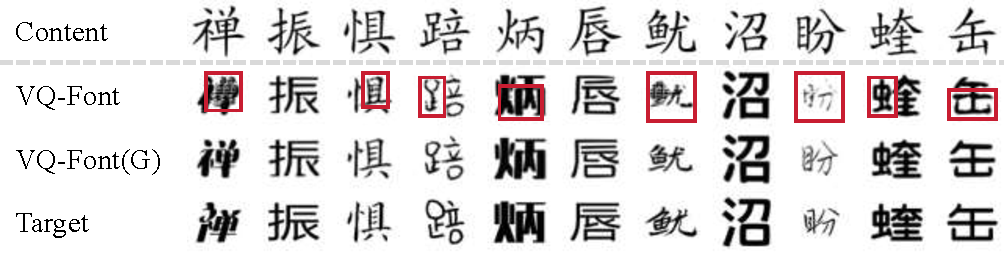
\includegraphics[width=0.95\linewidth]{SUPP_IMGS/EX_Visualization/VQ_G.pdf} 
  \caption{
Qualitative comparison on VQ-Font vs. VQ-Font (G). 
\textcolor{ex2figure_red}{\fbox{\rule{0pt}{4pt}\rule{4pt}{0pt}}} marks structural errors in the generated glyph. 
G-Tok improves structure preservation and produces more faithful font styles.
}
  \label{fig:supple_vq_g_ufuc}
\end{figure}


\begin{table*}[!t]
\centering
\caption{Quantitative evaluation of Multimodal FFG with full post-refinement (NFA and SE) on Unseen Fonts. All models listed are post-trained with NFA and SE stages on the Large dataset.}
\vspace{-2mm}
\setlength{\tabcolsep}{3pt}
\renewcommand{\arraystretch}{1.05}
\resizebox{0.95\textwidth}{!}{
\begin{tabular}{l | c c c c c c | c c c c c c }
\toprule
Method & \multicolumn{6}{c|}{Unseen Fonts Seen Characters (UFSC)} & \multicolumn{6}{c}{Unseen Fonts Unseen Characters (UFUC)} \\
\cmidrule(lr){2-7} \cmidrule(lr){8-13}
 & RMSE$\downarrow$ & SSIM$\uparrow$ & LPIPS$\downarrow$ & FID$\downarrow$ & Acc(C)$\uparrow$ & Acc(S)$\uparrow$
 & RMSE$\downarrow$ & SSIM$\uparrow$ & LPIPS$\downarrow$ & FID$\downarrow$ & Acc(C)$\uparrow$ & Acc(S)$\uparrow$ \\
\hline
$n_\text{ref}=2$ & 0.2501 & 0.6438 & 0.0888 & 10.1464 & \textbf{0.9851} & 0.3314 & 0.2701 & 0.5987 & 0.1069 & 9.4294 & 0.8720 & 0.3433 \\
$n_\text{ref}=4$ & 0.2437 & 0.6552 & 0.0848 & 9.5960  & 0.9839 & 0.3711 & 0.2692 & 0.6007 & 0.1049 & 9.0877 & 0.8828 & 0.3835 \\
$n_\text{ref}=8$ & 0.2398 & 0.6627 & 0.0831 & \textbf{8.3751}  & 0.9776 & 0.4154 & \textbf{0.2508} & \textbf{0.6377} & \textbf{0.0908} & \textbf{7.2034} & \textbf{0.9068} & 0.4183 \\
\Xhline{1.2pt}
GAR-Font($M_2$) & 0.2361 & 0.6707 & 0.0799 & 8.8867  & 0.9817 & 0.4508 & 0.2527 & 0.6352 & 0.0909 & 8.1444 & 0.9029 & 0.4247 \\
GAR-Font($M_4$) & \textbf{0.2358} & \textbf{0.6712} & \textbf{0.0796} & 8.8073  & 0.9800 & \textbf{0.4566} & 0.2524 & 0.6353 & \textbf{0.0908} & 8.0699 & 0.9023 & \textbf{0.4391} \\
\bottomrule
\end{tabular}
}
\label{tab:quant_eval_ref_mm}
\end{table*}
\begin{figure*}[!t]
    \centering
    \begin{minipage}{0.495\linewidth}
        \centering
        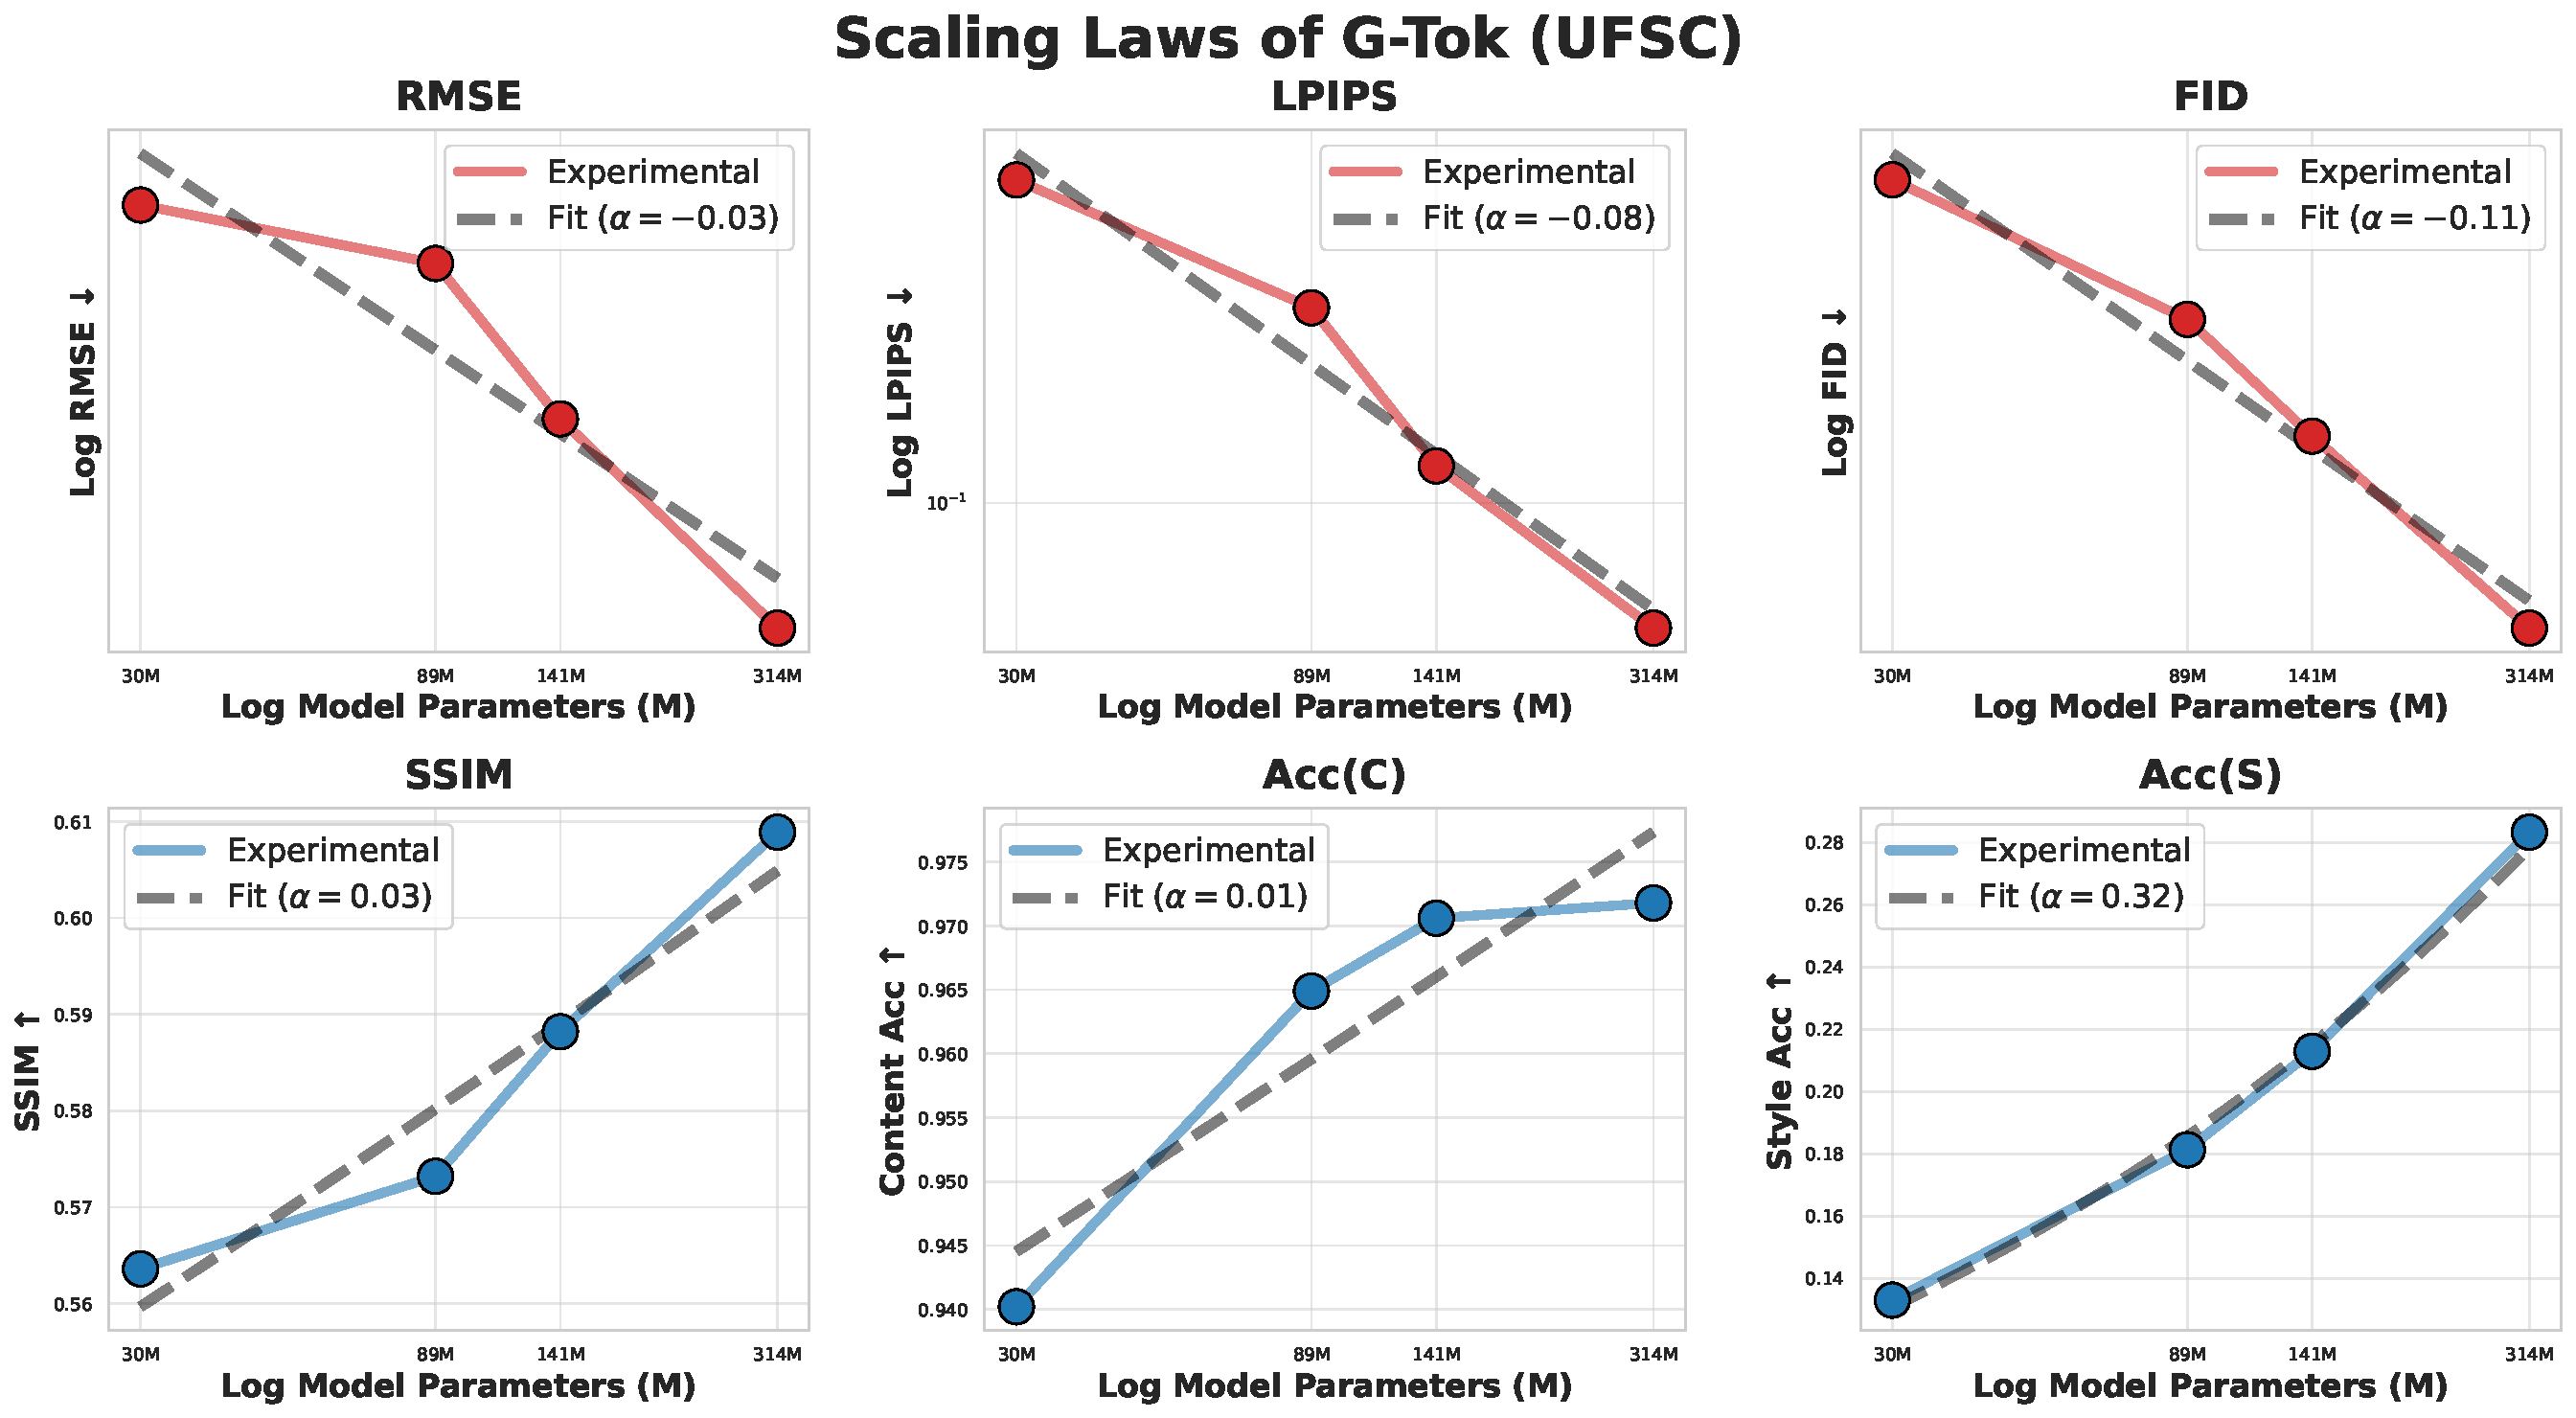
\includegraphics[width=\linewidth]{SUPP_IMGS/scaling_law_UFSC.pdf}
    \end{minipage}
    \hfill
    \begin{minipage}{0.495\linewidth}
        \centering
        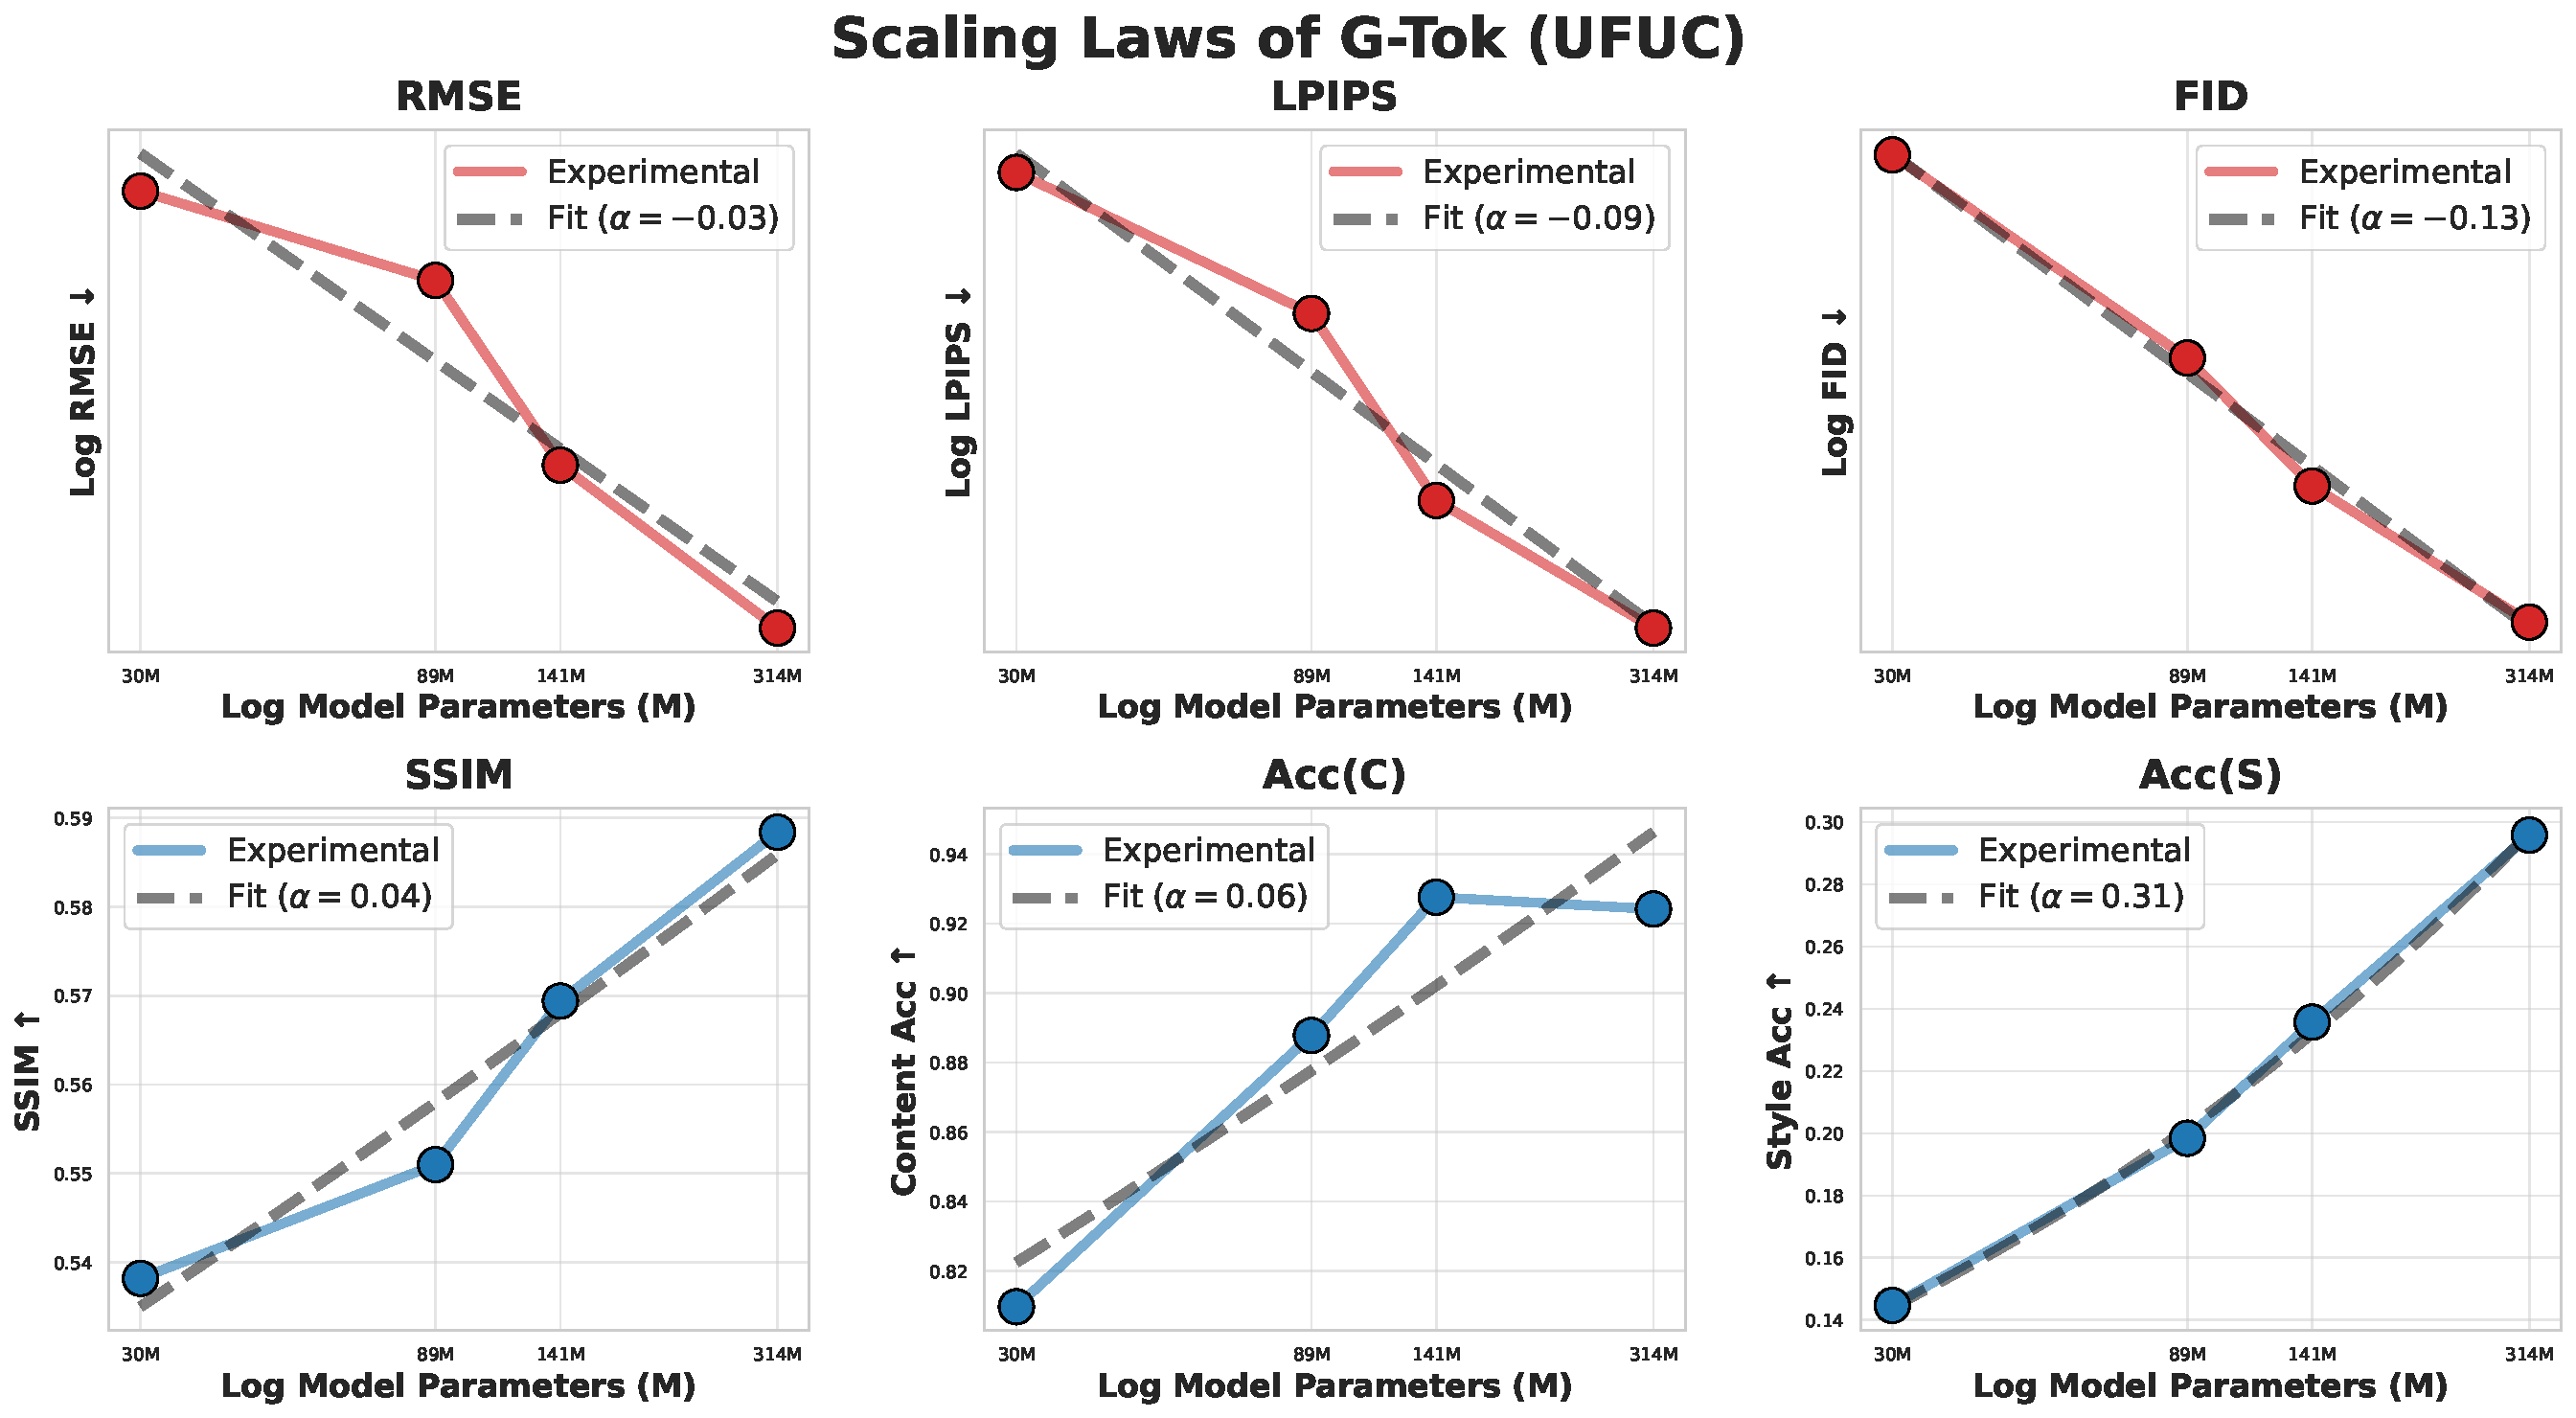
\includegraphics[width=\linewidth]{SUPP_IMGS/scaling_law_UFUC.pdf}
    \end{minipage}
    \vspace{-3mm}
    \caption{Scaling laws of the GAR-Font $(I_8)$ generator with NFA and SE refinement. The plots show performance metrics across model sizes (30M, 89M, 141M, 314M) on Unseen Fonts Seen Characters (\textit{UFSC}) and Unseen Fonts Unseen Characters (\textit{UFUC}). The dashed lines represent power-law fits, highlighting the predictable improvements in both perceptual quality and style generalization.}
    \vspace{-3mm}
    \label{fig:scaling_laws}
\end{figure*}
\subsection{Adaptation on G-Tok to Other FFG Methods}
\label{ssec:quantitiative_G-Tok_plugin}
To verify the versatility of our G-Tok, we integrated it into VQ-Font by replacing its native VQ-VAE with our G-Tok while maintaining the original model architecture and configuration. The modified model, \textbf{VQ-Font (G)}, was trained on the Small dataset with G-Tok. Due to time constraints, we trained it for only 150k iterations, compared with the 500k iterations used in the original VQ-Font. As shown in Table~\ref{tab:quant_eval_gtok_adaptation}, even under shorter training, this simple replacement yields significant improvements across all metrics. Most notably, FID$\downarrow$ decreases by nearly 50\% (e.g., $35.25 \to 17.33$ on \textit{UFSC}) and Content Accuracy$\uparrow$ improves by approximately 9\% ($\sim87\% \to \sim96\%$). These substantial gains demonstrate that G-Tok's hybrid CNN-ViT architecture captures far richer structural and stylistic semantics than standard VQ-VAEs, serving as a robust plug-and-play enhancement for quantization-based FFG methods. Figure~\ref{fig:supple_vq_g_ufuc} illustrates that integrating G-Tok helps the model preserve coherent global structures for complex fonts and generate styles that better align with the target font, indicating a richer and more semantically stable global representation G-Tok than the original VQ-VAE.


\subsection{Post-Refinement of Multimodal FFG}
\label{ssec:mm_post_refinement}

\begin{table*}[!t]
\centering
\caption{Quantitative evaluation of G-Tok's architecture on Unseen Fonts. All models listed are pre-trained on the Small dataset.}
\vspace{-2mm}
\setlength{\tabcolsep}{3pt}
\renewcommand{\arraystretch}{1.05}
\resizebox{0.95\textwidth}{!}{
\begin{tabular}{l | c c c c c c | c c c c c c }
\toprule
Method & \multicolumn{6}{c|}{Unseen Fonts Seen Characters (UFSC)} & \multicolumn{6}{c}{Unseen Fonts Unseen Characters (UFUC)} \\
\cmidrule(lr){2-7} \cmidrule(lr){8-13}
 & RMSE$\downarrow$ & SSIM$\uparrow$ & LPIPS$\downarrow$ & FID$\downarrow$ & Acc(C)$\uparrow$ & Acc(S)$\uparrow$ 
 & RMSE$\downarrow$ & SSIM$\uparrow$ & LPIPS$\downarrow$ & FID$\downarrow$ & Acc(C)$\uparrow$ & Acc(S)$\uparrow$ \\
\hline
CNN & 0.3212 & 0.4836 & 0.1442 & 9.5071 & 0.9051 & 0.0235 & 0.3447 & 0.4350 & 0.1728 & 10.5239 & 0.6722 & 0.0221 \\
CNN+Non-Causal ViT & 0.3183 & 0.4919 & 0.1458 & \textbf{7.9101} & 0.9268 & 0.0402 & 0.3271 & 0.4745 & 0.1562 & 8.7504 & 0.8019 & 0.0436 \\
CNN+Causal ViT & \textbf{0.3080} & \textbf{0.5052} & \textbf{0.1313} & 7.9484 & \textbf{0.9408} & \textbf{0.0802} & \textbf{0.3142} & \textbf{0.4932} & \textbf{0.1421} & \textbf{8.4841} & \textbf{0.8993} & \textbf{0.0796} \\
\bottomrule
\end{tabular}
}
\label{tab:ablation_gtok_generator}
\end{table*}

In Section 4.4, we demonstrated the efficacy of G-Tok$(M_2/M_4)$ on multimodal FFG, but limited to pretraining stage. To fully assess the potential of our lightweight vision-language adaptation, we extend the evaluation to the complete pipeline. We apply our post-training NFA and SE stages to both the vision-only baselines and our multimodal variants. All models are trained on the Large (\textit{L}) dataset.

As visualized in Table~\ref{tab:quant_eval_ref_mm}, the inclusion of textual descriptions significantly enhances the effectiveness of the post-refinement stage. Unlike the pre-training phase where multimodal models showed a slight dip in style accuracy (Acc(S)$\uparrow$), the fully refined GAR-Font($M_2$) and GAR-Font($M_4$) exhibit a substantial lead in Acc(S)$\uparrow$ compared to their vision-only counterparts ($n_\text{ref}=2$ and $n_\text{ref}=4$). Notably, \textbf{GAR-Font($M_4$) outperforms the 8-reference vision-only baseline ($n_\text{ref}=8$)} across most key metrics, including RMSE$\downarrow$, SSIM$\uparrow$, LPIPS$\downarrow$, and Style Accuracy$\uparrow$ (0.4566 vs. 0.4154 on \textit{UFSC}).


\subsection{Scaling Laws of GAR-Font\texorpdfstring{$(I_8)$}{(I8)}}
\label{ssec:scaling_law}
We evaluate the scalability of GAR-Font$(I_8)$ with NFA and SE on the small dataset by training models from 30M to 314M parameters and measuring performance across standard quantitative metrics. Following established scaling-law formulations, we model the relationship between model size $N$ and loss metric $L$ using a power law $L(N)\propto N^{-\alpha}$, and analyze trends in log–log space, where an ideal scaling law appears linear and the slope $\alpha$ reflects scaling efficiency.

As shown in Figure~\ref{fig:scaling_laws}, the enhanced GAR-Font models closely follow these power-law predictions, exhibiting smooth, monotonic improvements across all metrics. Loss-based metrics (FID$\downarrow$, LPIPS$\downarrow$, RMSE$\downarrow$) scale linearly with negative slopes, with FID$\downarrow$ showing a pronounced gain, indicating that larger models continue to yield substantial perceptual improvements without saturation. Accuracy metrics display complementary behavior: Content Accuracy (Acc(C)$\uparrow$) saturates early due to task simplicity, whereas Style Accuracy (Acc(S)$\uparrow$) benefits most from increased capacity. This steep scaling trend highlights that NFA and SE effectively exploit larger parameter budgets to capture and generalize complex stylistic attributes, underscoring the central role of scale in high-fidelity font generation.





% \subsection{Post-Refinement of GAR-Font\texorpdfstring{$(M_2/M_4)$}{(M2/M4)}}

% To fully explore the potential of our lightweight language-style adaptation, we apply the complete post-refinement pipeline (NFA and SE) to GAR-Font($M_2$) and GAR-Font($M_4$). 

% \begin{table*}[t]
% \centering
% \caption{Quantitative evaluation on unseen fonts (MM Post-Refinement train on Large).}
% \vspace{-2mm}
% \setlength{\tabcolsep}{3pt}
% \renewcommand{\arraystretch}{1.05}
% \resizebox{0.95\textwidth}{!}{
% \begin{tabular}{l | c c c c c c | c c c c c c }
% \toprule
% Method & \multicolumn{6}{c|}{Unseen Fonts Seen Characters (UFSC)} & \multicolumn{6}{c}{Unseen Fonts Unseen Characters (UFUC)} \\
% \cmidrule(lr){2-7} \cmidrule(lr){8-13}
%  & RMSE$\downarrow$ & SSIM$\uparrow$ & LPIPS$\downarrow$ & FID$\downarrow$ & Acc(C)$\uparrow$ & Acc(S)$\uparrow$
%  & RMSE$\downarrow$ & SSIM$\uparrow$ & LPIPS$\downarrow$ & FID$\downarrow$ & Acc(C)$\uparrow$ & Acc(S)$\uparrow$ \\
% \hline
% I8\_NFA\_SE\_ref2   & 0.2501 & 0.6438 & 0.0888 & 10.1464 & \textbf{0.9851} & 0.3314 & 0.2701 & 0.5987 & 0.1069 & 9.4294 & 0.8720 & 0.3433 \\
% I8\_NFA\_SE\_ref4   & 0.2437 & 0.6552 & 0.0848 & 9.5960  & 0.9839 & 0.3711 & 0.2692 & 0.6007 & 0.1049 & 9.0877 & 0.8828 & 0.3835 \\
% I8\_NFA\_SE\_ref8   & 0.2398 & 0.6627 & 0.0831 & \textbf{8.3751}  & 0.9776 & 0.4154 & \textbf{0.2508} & \textbf{0.6377} & \textbf{0.0908} & \textbf{7.2034} & \textbf{0.9068} & 0.4183 \\
% MM2\_NFA\_SE        & 0.2361 & 0.6707 & 0.0799 & 8.8867  & 0.9817 & 0.4508 & 0.2527 & 0.6352 & 0.0909 & 8.1444 & 0.9029 & 0.4247 \\
% MM4\_NFA\_SE        & \textbf{0.2358} & \textbf{0.6712} & \textbf{0.0796} & 8.8073  & 0.9800 & \textbf{0.4566} & 0.2524 & 0.6353 & 0.0908 & 8.0699 & 0.9023 & \textbf{0.4391} \\
% \bottomrule
% \end{tabular}
% }
% \label{tab:quant_eval_ref_mm}
% \end{table*}
% \begin{table*}[t]
% \centering
% \caption{Quantitative evaluation on unseen fonts (VQ-Font vs VQ-Font (G).}
% \vspace{-2mm}
% \setlength{\tabcolsep}{3pt}
% \renewcommand{\arraystretch}{1.05}
% \resizebox{0.95\textwidth}{!}{
% \begin{tabular}{l | c c c c c c | c c c c c c }
% \toprule
% Method & \multicolumn{6}{c|}{Unseen Fonts Seen Characters (UFSC)} & \multicolumn{6}{c}{Unseen Fonts Unseen Characters (UFUC)} \\
% \cmidrule(lr){2-7} \cmidrule(lr){8-13}
%  & RMSE$\downarrow$ & SSIM$\uparrow$ & LPIPS$\downarrow$ & FID$\downarrow$ & Acc(C)$\uparrow$ & Acc(S)$\uparrow$
%  & RMSE$\downarrow$ & SSIM$\uparrow$ & LPIPS$\downarrow$ & FID$\downarrow$ & Acc(C)$\uparrow$ & Acc(S)$\uparrow$ \\
% \hline
% VQ\_Font & 0.2727 & 0.5642 & 0.1830 & 35.2472 & 0.8763 & 0.0016 & 0.2744 & 0.5616 & 0.1822 & 36.7914 & 0.8882 & 0.0016 \\
% VQ\_Font (G)   & 0.2725 & 0.5644 & 0.1731 & 17.3296  & 0.9646 & 0.0022 & - & - & - & - &- &- \\
% \bottomrule
% \end{tabular}
% }
% \label{tab:quant_eval_ref_mm}
% \end{table*}


% \subsection{Scaling Laws of GAR-Font$(I_8)$}
% 340M, 150M, 90M, 50M
% To explore how model capacity affects autoregressive font generation, we conduct an additional scaling study on the AR Generator using the Small dataset. We train models of varying sizes and evaluate them across the full set of quantitative metrics, reported in Table~S\_X. The results show a consistent monotonic improvement with increasing model size, demonstrating a clear scaling trend for AR-based glyph modeling.
% \begin{table*}[t]
% \centering
% \caption{Quantitative evaluation on unseen fonts. (Scaling Law, Train on Small)}
% \vspace{-2mm}
% \setlength{\tabcolsep}{3pt}
% \renewcommand{\arraystretch}{1.05}
% \resizebox{0.95\textwidth}{!}{
% \begin{tabular}{l | c c c c c c | c c c c c c }
% \toprule
% Method & \multicolumn{6}{c|}{Unseen Fonts Seen Characters (UFSC)} & \multicolumn{6}{c}{Unseen Fonts Unseen Characters (UFUC)} \\
% \cmidrule(lr){2-7} \cmidrule(lr){8-13}
%  & RMSE$\downarrow$ & SSIM$\uparrow$ & LPIPS$\downarrow$ & FID$\downarrow$ & Acc(C)$\uparrow$ & Acc(S)$\uparrow$
%  & RMSE$\downarrow$ & SSIM$\uparrow$ & LPIPS$\downarrow$ & FID$\downarrow$ & Acc(C)$\uparrow$ & Acc(S)$\uparrow$ \\
% \hline
% 50M\_Pre & 0.3234 & 0.4803 & 0.1478 & 9.5682 & 0.9002 & 0.0347 & 0.3233 & 0.4826 & 0.1473 & 9.8740 & 0.8878 & 0.0375 \\
% 90M\_Pre & 0.3219 & 0.4879 & 0.1409 & 7.9230 & 0.9220 & 0.0448 & 0.3212 & 0.4911 & 0.1409 & 8.1393 & 0.9094 & 0.0502 \\
% 150M\_Pre & 0.3212 & 0.4845 & 0.1449 & 7.9945 & 0.9297 & 0.0471 & 0.3210 & 0.4864 & 0.1449 & 8.4493 & 0.9281 & 0.0506 \\
% 340M\_Pre & 0.3080 & 0.5052 & 0.1313 & 7.9484 & 0.9408 & 0.0802 & 0.3142 & 0.4932 & 0.1421 & 8.4841 & 0.8993 & 0.0796 \\
% \hline
% 50M\_NFA & 0.2977 & 0.5280 & 0.1241 & 10.0811 & 0.7837 & 0.1026 & 0.2979 & 0.5293 & 0.1235 & 10.2685 & 0.7455 & 0.1234 \\
% 90M\_NFA & 0.2937 & 0.5404 & 0.1172 & 7.7879 & 0.8371 & 0.1549 & 0.2928 & 0.5441 & 0.1164 & 7.8355 & 0.8124 & 0.1766 \\
% 150M\_NFA & 0.2874 & 0.5563 & 0.1107 & 6.5190 & 0.8599 & 0.2009 & 0.2862 & 0.5602 & 0.1094 & 6.7234 & 0.8448 & 0.2208 \\
% 340M\_NFA & 0.2712 & 0.5933 & 0.0992 & \textbf{5.4254} & 0.9236 & \textbf{0.3179} & 0.2836 & 0.5702 & 0.1079 & \textbf{5.6667} & 0.8817 & \textbf{0.3277} \\
% \hline
% 50M\_NFA\_SE & 0.2854 & 0.5636 & 0.1148 & 8.9481 & 0.9402 & 0.1330 & 0.2988 & 0.5382 & 0.1257 & 9.6713 & 0.8097 & 0.1447 \\
% 90M\_NFA\_SE & 0.2828 & 0.5732 & 0.1087 & 8.2565 & 0.9649 & 0.1813 & 0.2946 & 0.5510 & 0.1179 & 8.4715 & 0.8878 & 0.1984 \\
% 150M\_NFA\_SE & 0.2760 & 0.5882 & 0.1016 & 7.7190 & 0.9706 & 0.2129 & 0.2861 & 0.5694 & 0.1083 & 7.7930 & 0.9276 & 0.2357 \\
% 340M\_NFA\_SE & \textbf{0.2671} & \textbf{0.6089} & \textbf{0.0948} & 6.9103 & \textbf{0.9718} & 0.2833 & \textbf{0.2788} & \textbf{0.5884} & \textbf{0.1022} & 7.1309 & \textbf{0.9242} & 0.2958 \\
% \bottomrule
% \end{tabular}
% }
% \label{tab:quant_eval_fonts}
% \end{table*}



\section{Additional Ablative Studies}
\label{sec:Ablate}
\subsection{On G-Tok's hybrid Architecture}
% Reconstruction results (0.2 0.2)
To further illustrate the robustness of our hybrid CNN–ViT tokenizer, we provide complete visualizations of the \textbf{Reconstruction Robustness} experiment, where glyphs are corrupted with localized Gaussian noise ($\sigma = 0.2$, affecting 20\% area).  
The qualitative results in Figure~\ref{fig:supple_abl1_rec} demonstrate that G-Tok robustly recovers structural layout and stylistic traits even under severe perturbations, while non-hybrid alternatives fail to reconstruct consistent structure. 

% This visual evidence complements the quantitative robustness results in Section~5.3.

\subsection{On G-Tok's Global and Causal Modeling}
% UFSC,  UFUC,  Small dataset
We present full ablation results for the global and causal modeling components of G-Tok.  
Table ~\ref{tab:ablation_gtok_generator} reports the complete quantitative comparison on the \textit{UFSC/UFUC}. As discussed in Section~5.3, adding global self-attention (CNN + Non-causal ViT) significantly outperforms the CNN-only baseline, while the causal ViT further improves sequential modeling and yields the best overall performance.


Figure ~\ref{fig: supple_abl2_all} provides qualitative comparisons on (\textit{UFSC}, Small) and (\textit{UFUC}, Small). The AR Generator implemented with a CNN-only tokenizer often exhibits style mismatches and inconsistent strokes. Introducing ViT modules into the tokenizer enhances its ability to perceive and capture global stylistic context, leading to more coherent font generation. The AR variant with full G-Tok (CNN + Causal ViT) achieves the most robust performance, showing visible improvements in stylistic and  structural fidelity.

\subsection{On AR Generator's Soft-Decoding}
We provide full visualizations to assess the impact of pixel-level supervision and the soft-decoding strategy. As shown in Figure~\ref{fig: supple_abl3_all} under both (\textit{UFSC}, Small) and (\textit{UFUC}, Small), pixel-level supervision enhances structural accuracy, while soft decoding yields smoother, more continuous strokes and reduces broken segments and visual artifacts.



\begin{figure}[t]
  \centering
  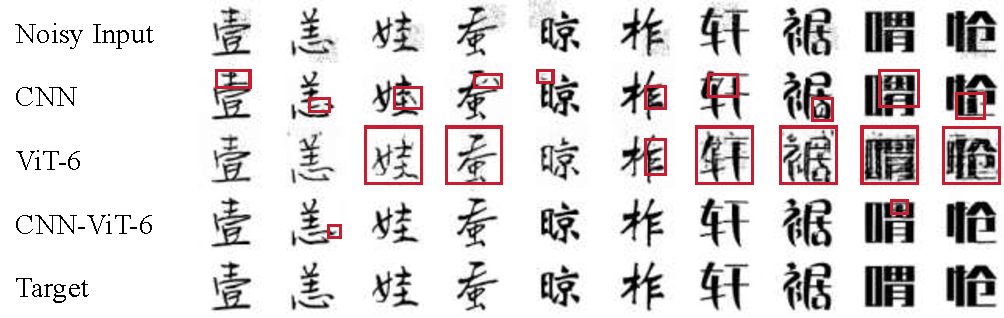
\includegraphics[width=0.95\linewidth]{SUPP_IMGS/EX_Visualization/ABL1_Rec.pdf} 
  \vspace{-3mm}
  \caption{Reconstruction Robustness under localized Gaussian noise ($\sigma = 0.2$, 20\% area). \textcolor{ex2figure_red}{\fbox{\rule{0pt}{4pt}\rule{4pt}{0pt}}} marks structural mistakes. G-Tok maintains structural and stylistic fidelity despite heavy corruption, while non-hybrid tokenizers exhibit unstable and inconsistent reconstructions.}
  \vspace{-3mm}
  \label{fig:supple_abl1_rec}
\end{figure}

\begin{figure*}[tp] % [p] 强制将这些内容放在单独的一页
    \centering
    
    % ================== 第一组图 (G-Tok) ==================
    \begin{subfigure}{0.93\linewidth} % 尝试缩小到 0.8 或 0.75
        \centering
        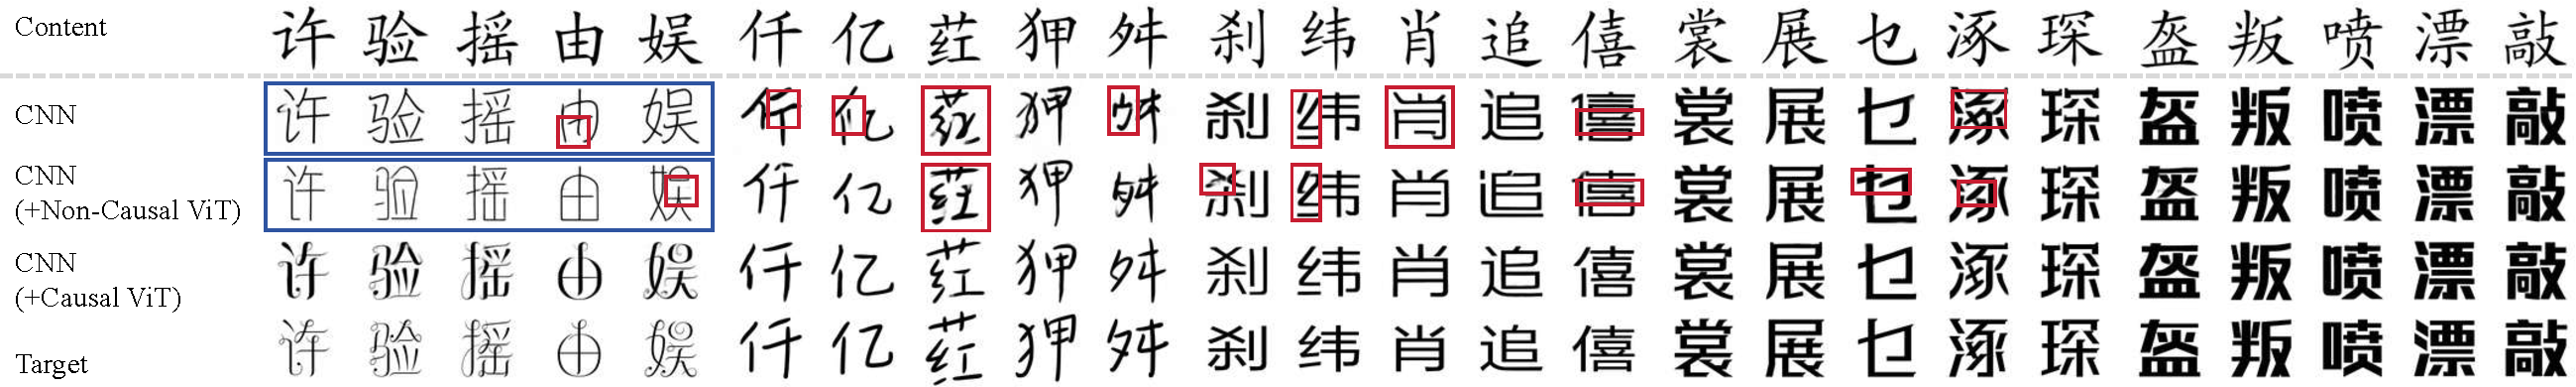
\includegraphics[width=\linewidth]{SUPP_IMGS/EX_Visualization/ABL2_table_UFSC_Small.pdf}
        \caption{\textit{UFSC}, Small dataset}
        \label{fig: supple_abl2_ufsc_small}
    \end{subfigure}
    \\ % 强制换行，确保垂直排列
    \begin{subfigure}{0.93\linewidth}
        \centering
        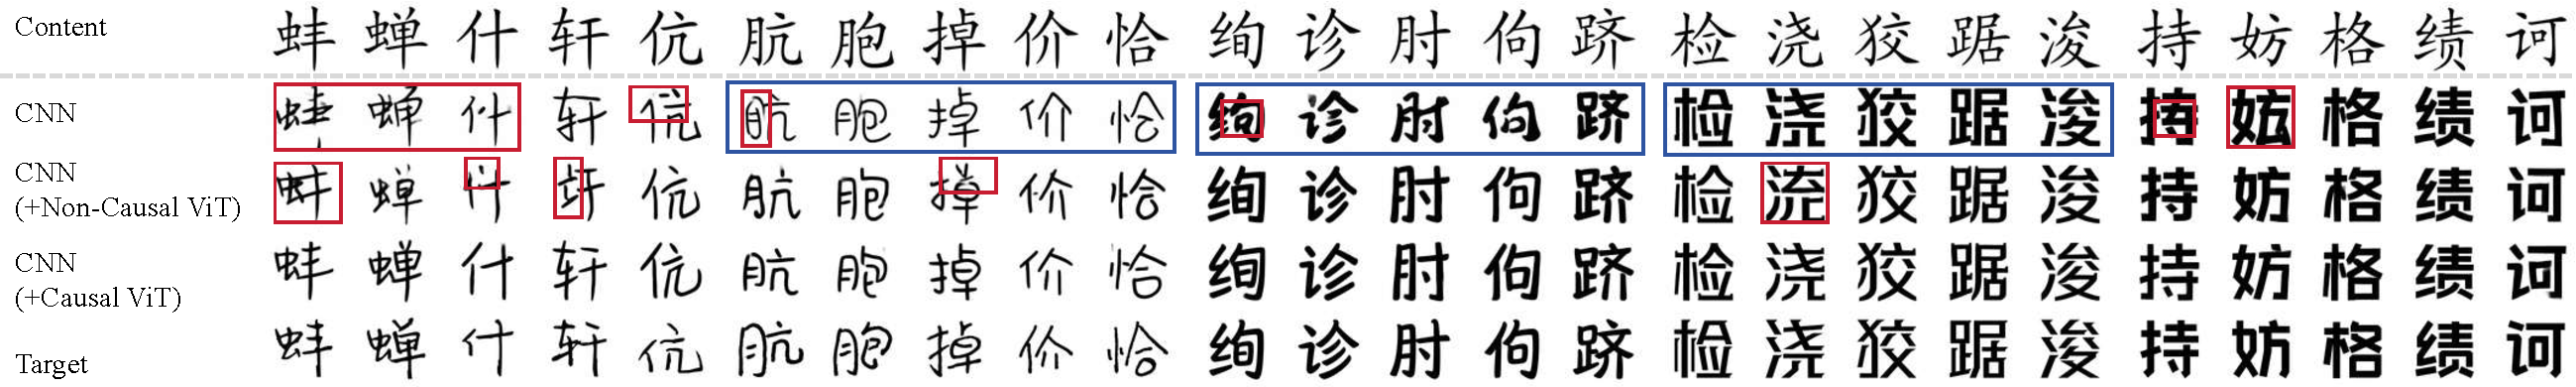
\includegraphics[width=\linewidth]{SUPP_IMGS/EX_Visualization/ABL2_table_UFUC_Small.pdf}
        \caption{\textit{UFUC}, Small dataset}
        \label{fig: supple_abl2_ufuc_small}
    \end{subfigure}
    \vspace{-3mm}
    \caption{Qualitative results on G-Tok's Global and Causal Modeling under \textit{UFSC} and \textit{UFUC} protocols
        (Small dataset). 
        \textcolor{ex1figure_red}{\fbox{\rule{0pt}{4pt}\rule{4pt}{0pt}}} /
        \textcolor{ex1figure_blue}{\fbox{\rule{0pt}{4pt}\rule{4pt}{0pt}}}
        indicate structural errors and style mismatches.}
    \label{fig: supple_abl2_all}
    
    \vspace{1em} % 在不同 Figure 之间增加一点区分距离
    
    % ================== 第二组图 (AR Generator) ==================
    \begin{subfigure}{0.93\linewidth}
        \centering
        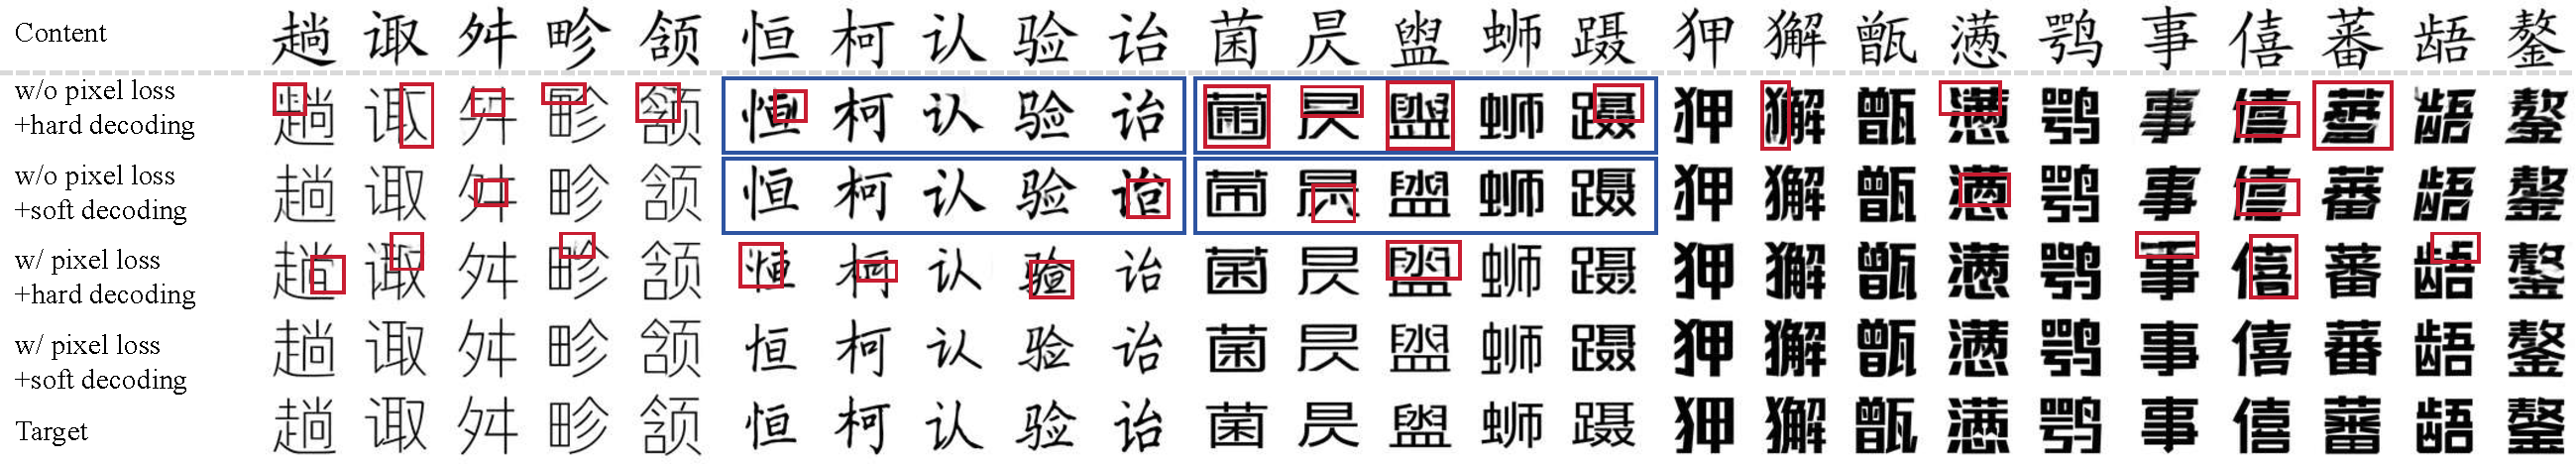
\includegraphics[width=\linewidth]{SUPP_IMGS/EX_Visualization/ABL3_Table_UFSC_Small.pdf}
        \caption{\textit{UFSC}, Small dataset}
        \label{fig: supple_abl3_ufsc_small}
    \end{subfigure}
    \\
    \begin{subfigure}{0.93\linewidth}
        \centering
        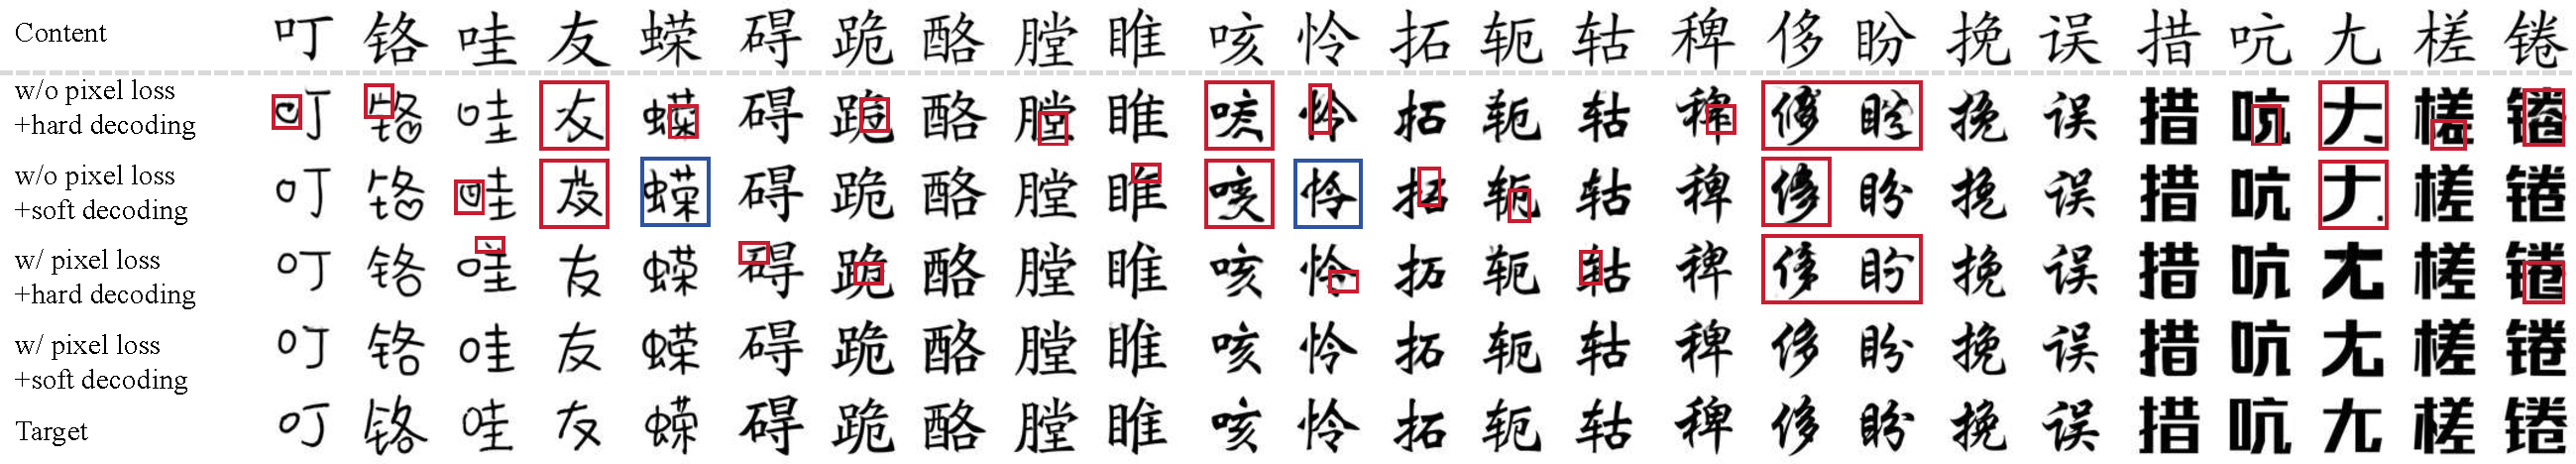
\includegraphics[width=\linewidth]{SUPP_IMGS/EX_Visualization/ABL3_Table_UFUC_Small.pdf}
        \caption{\textit{UFUC}, Small dataset}
        \label{fig: supple_abl3_ufuc_small}
    \end{subfigure}
    \vspace{-3mm}
    \caption{Qualitative results on AR Generator's Soft-decoding under \textit{UFSC} and \textit{UFUC} protocols
        (Small dataset).
        \textcolor{ex1figure_red}{\fbox{\rule{0pt}{4pt}\rule{4pt}{0pt}}} /
        \textcolor{ex1figure_blue}{\fbox{\rule{0pt}{4pt}\rule{4pt}{0pt}}}
        indicate structural errors and style mismatches.}
    \label{fig: supple_abl3_all}

    \vspace{1em}

    % ================== 第三组图 (Multimodal Style) ==================
    \begin{subfigure}{0.93\linewidth}
        \centering
        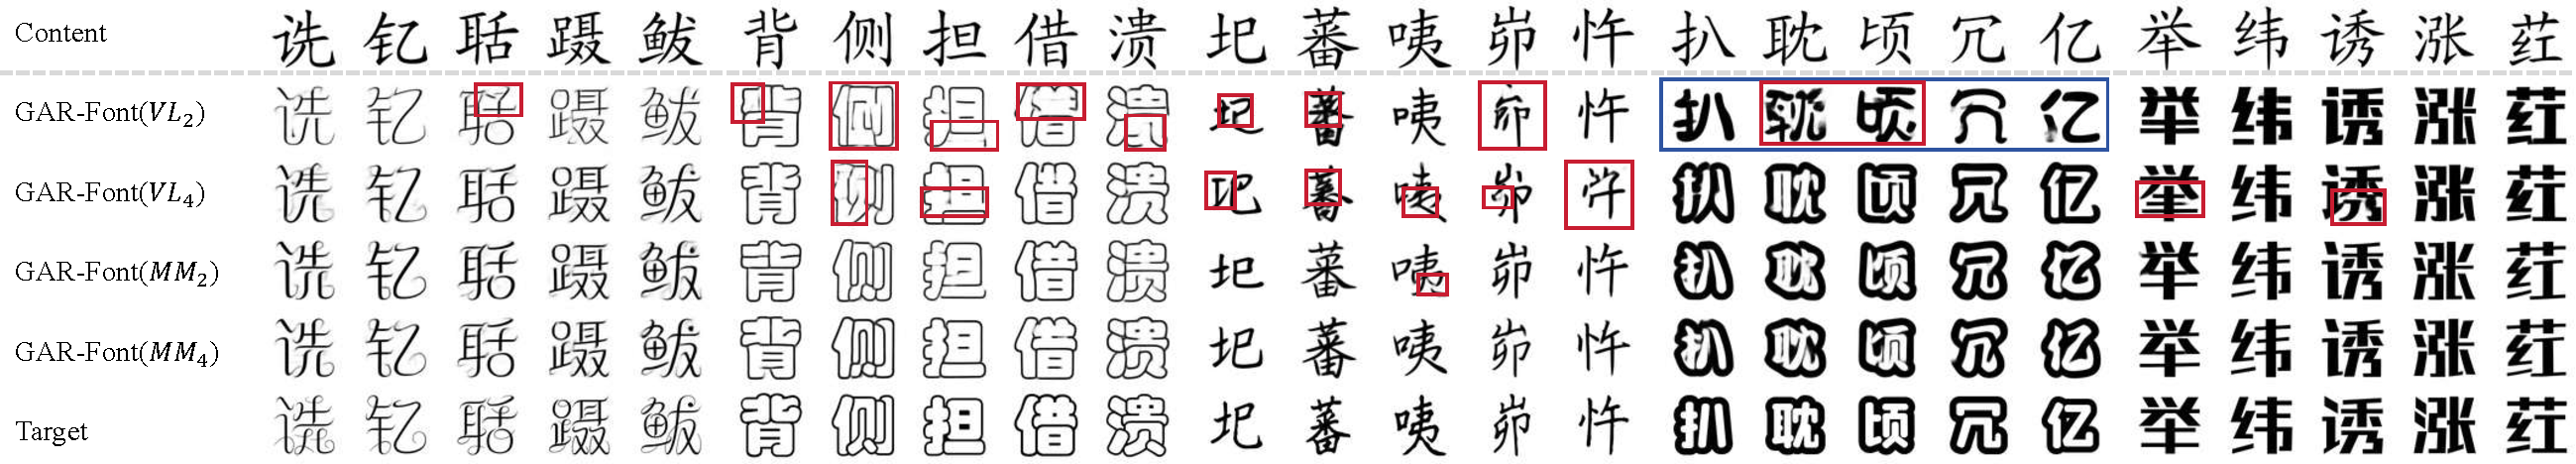
\includegraphics[width=\linewidth]{SUPP_IMGS/EX_Visualization/ABL4_Table_UFSC_Large.pdf}
        \caption{\textit{UFSC}, Large dataset}
        \label{fig: supple_abl4_ufsc_large}
    \end{subfigure}
    \\
    \begin{subfigure}{0.93\linewidth}
        \centering
        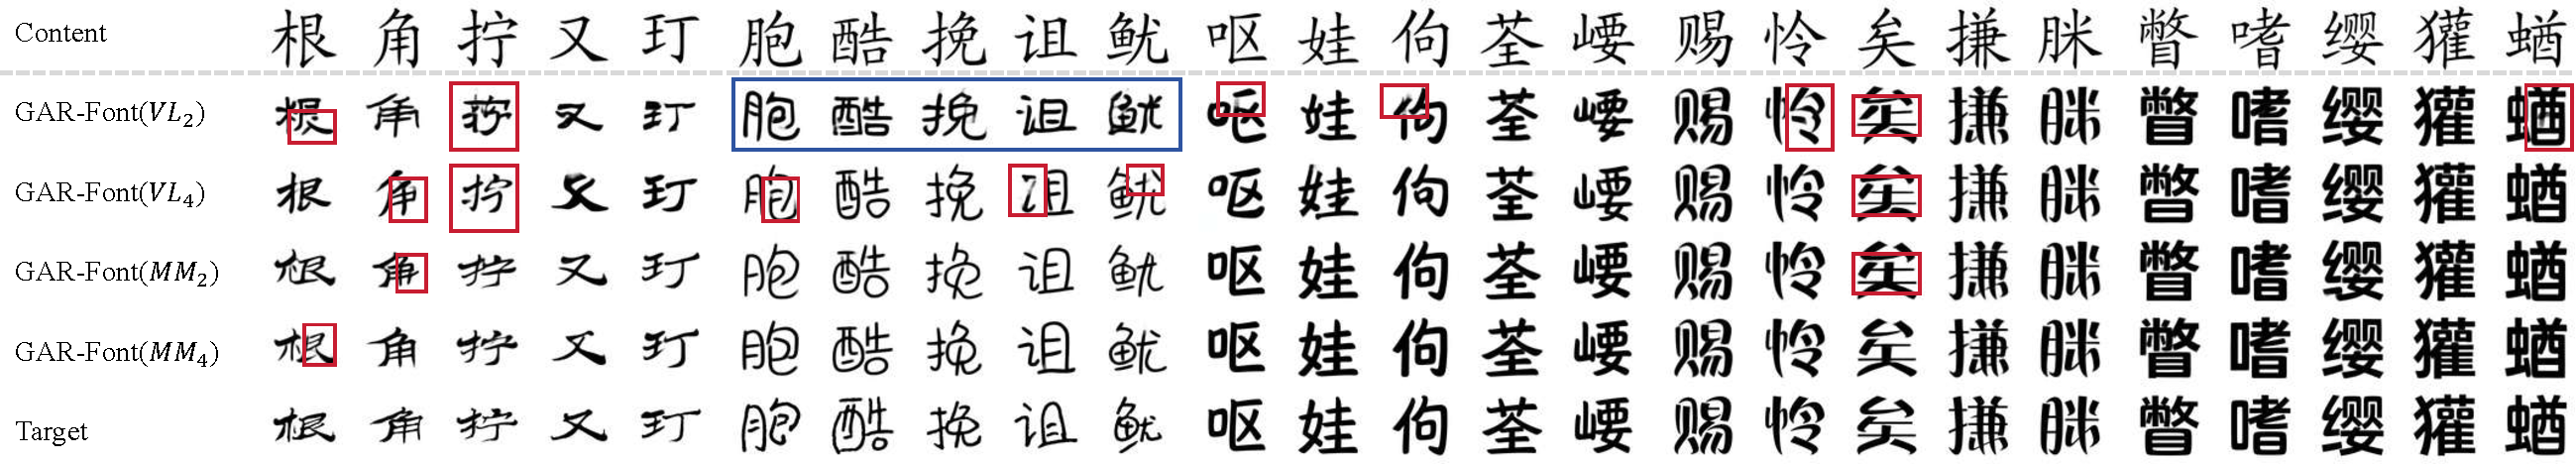
\includegraphics[width=\linewidth]{SUPP_IMGS/EX_Visualization/ABL4_Table_UFUC_Large.pdf}
        \caption{\textit{UFUC}, Large dataset}
        \label{fig: supple_abl4_ufuc_large}
    \end{subfigure}
    \vspace{-3mm}
    \caption{
        Qualitative results on Multimodal Style Encoder's Adaptation under \textit{UFSC} and \textit{UFUC} protocols
        (Large dataset).
        \textcolor{ex1figure_red}{\fbox{\rule{0pt}{4pt}\rule{4pt}{0pt}}} /
        \textcolor{ex1figure_blue}{\fbox{\rule{0pt}{4pt}\rule{4pt}{0pt}}}
        indicate structural errors and style mismatches.
    }
    \label{fig: supple_abl4_all}
    
\end{figure*}
\begin{figure*}[tp]
    \centering

    \begin{subfigure}{0.91\linewidth}
        \centering
        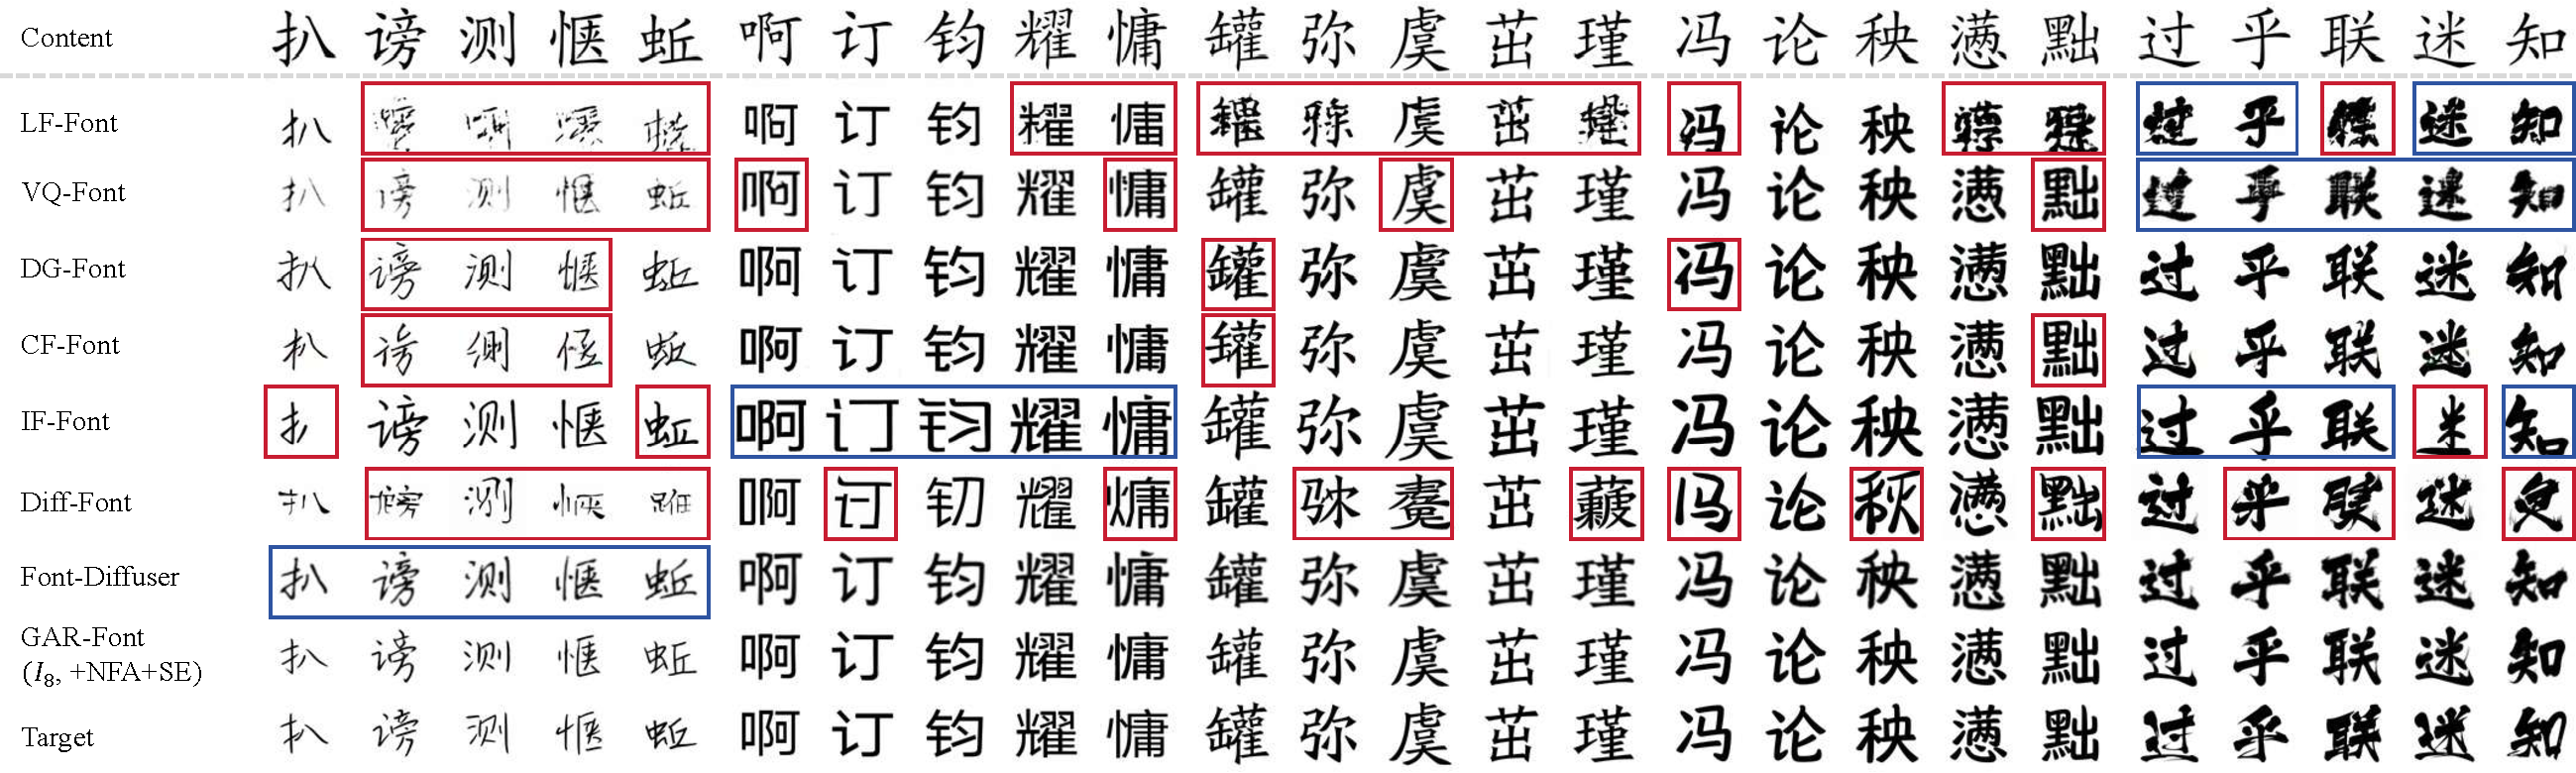
\includegraphics[width=\linewidth]{SUPP_IMGS/EX_Visualization/table_Main1_UFSC_Small.pdf}
        \vspace{-3mm}
        \caption{\textit{UFSC}, Small dataset}
        \label{fig: supple_main1_ufsc_small}
        \vspace{1mm}
    \end{subfigure}

    \begin{subfigure}{0.91\linewidth}
        \centering
        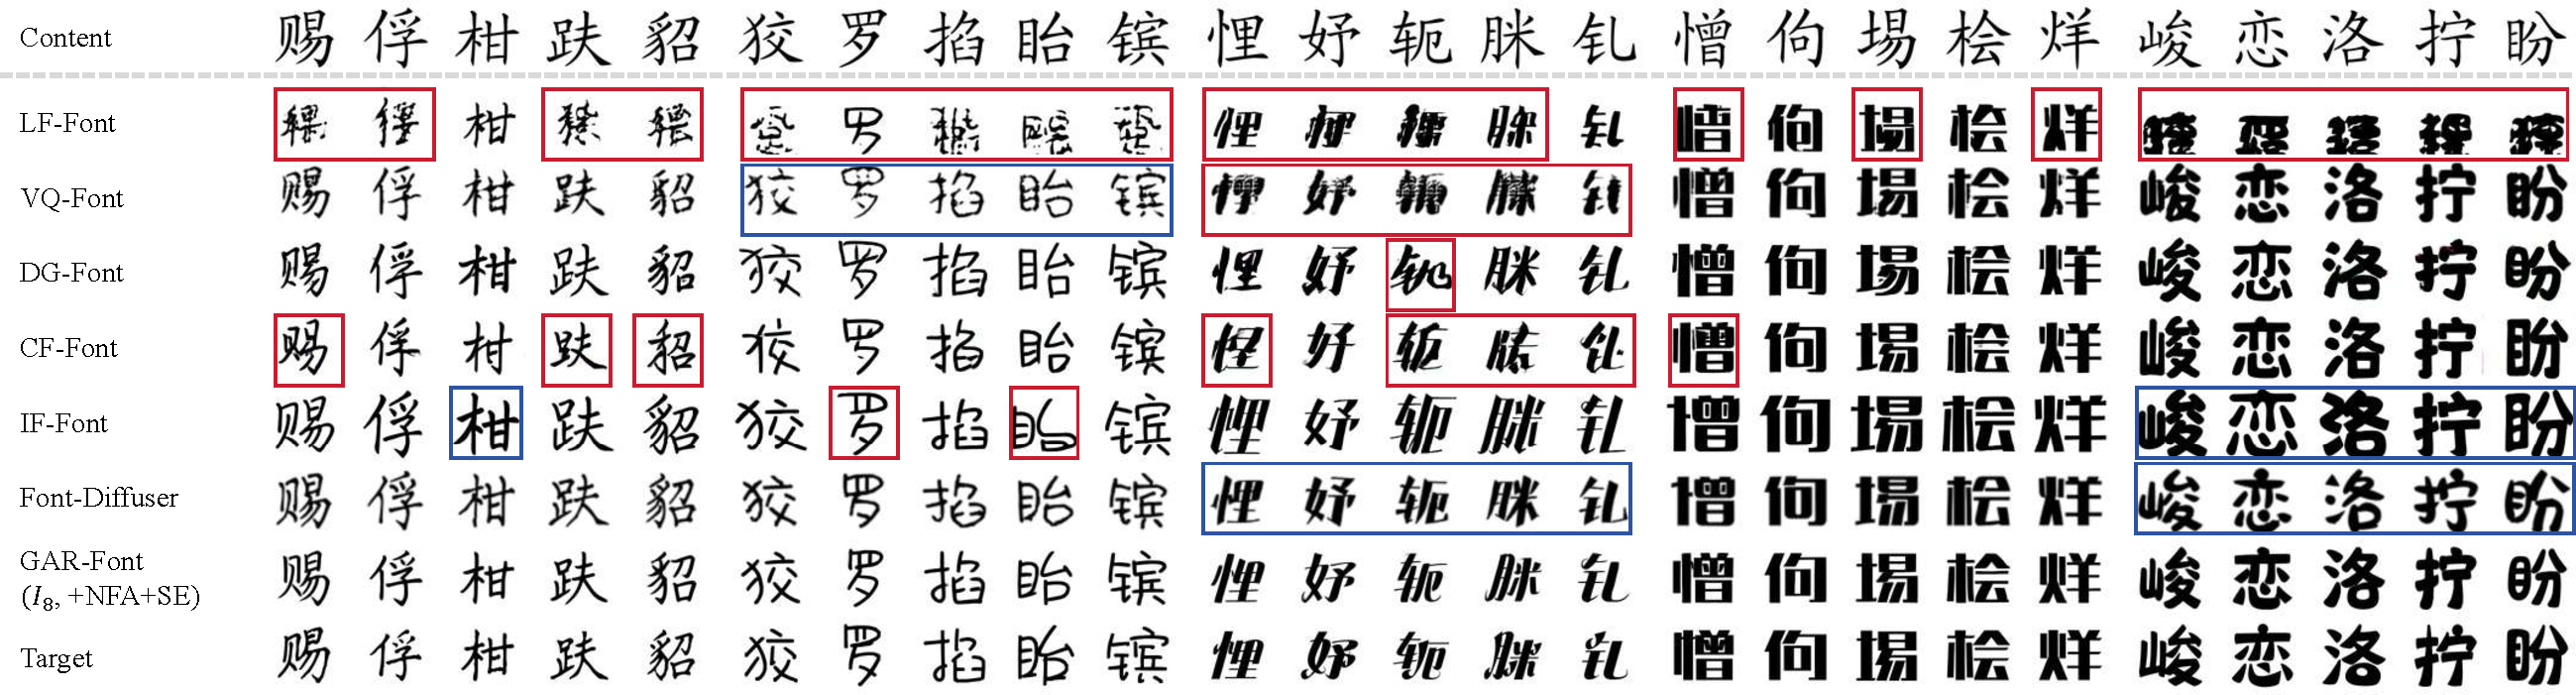
\includegraphics[width=\linewidth]{SUPP_IMGS/EX_Visualization/table_Main1_UFUC_Small.pdf}
        \vspace{-3mm}
        \caption{\textit{UFUC}, Small dataset}
        \vspace{1mm}
        \label{fig: supple_main1_ufuc_small}
    \end{subfigure}

    \begin{subfigure}{0.91\linewidth}
        \centering
        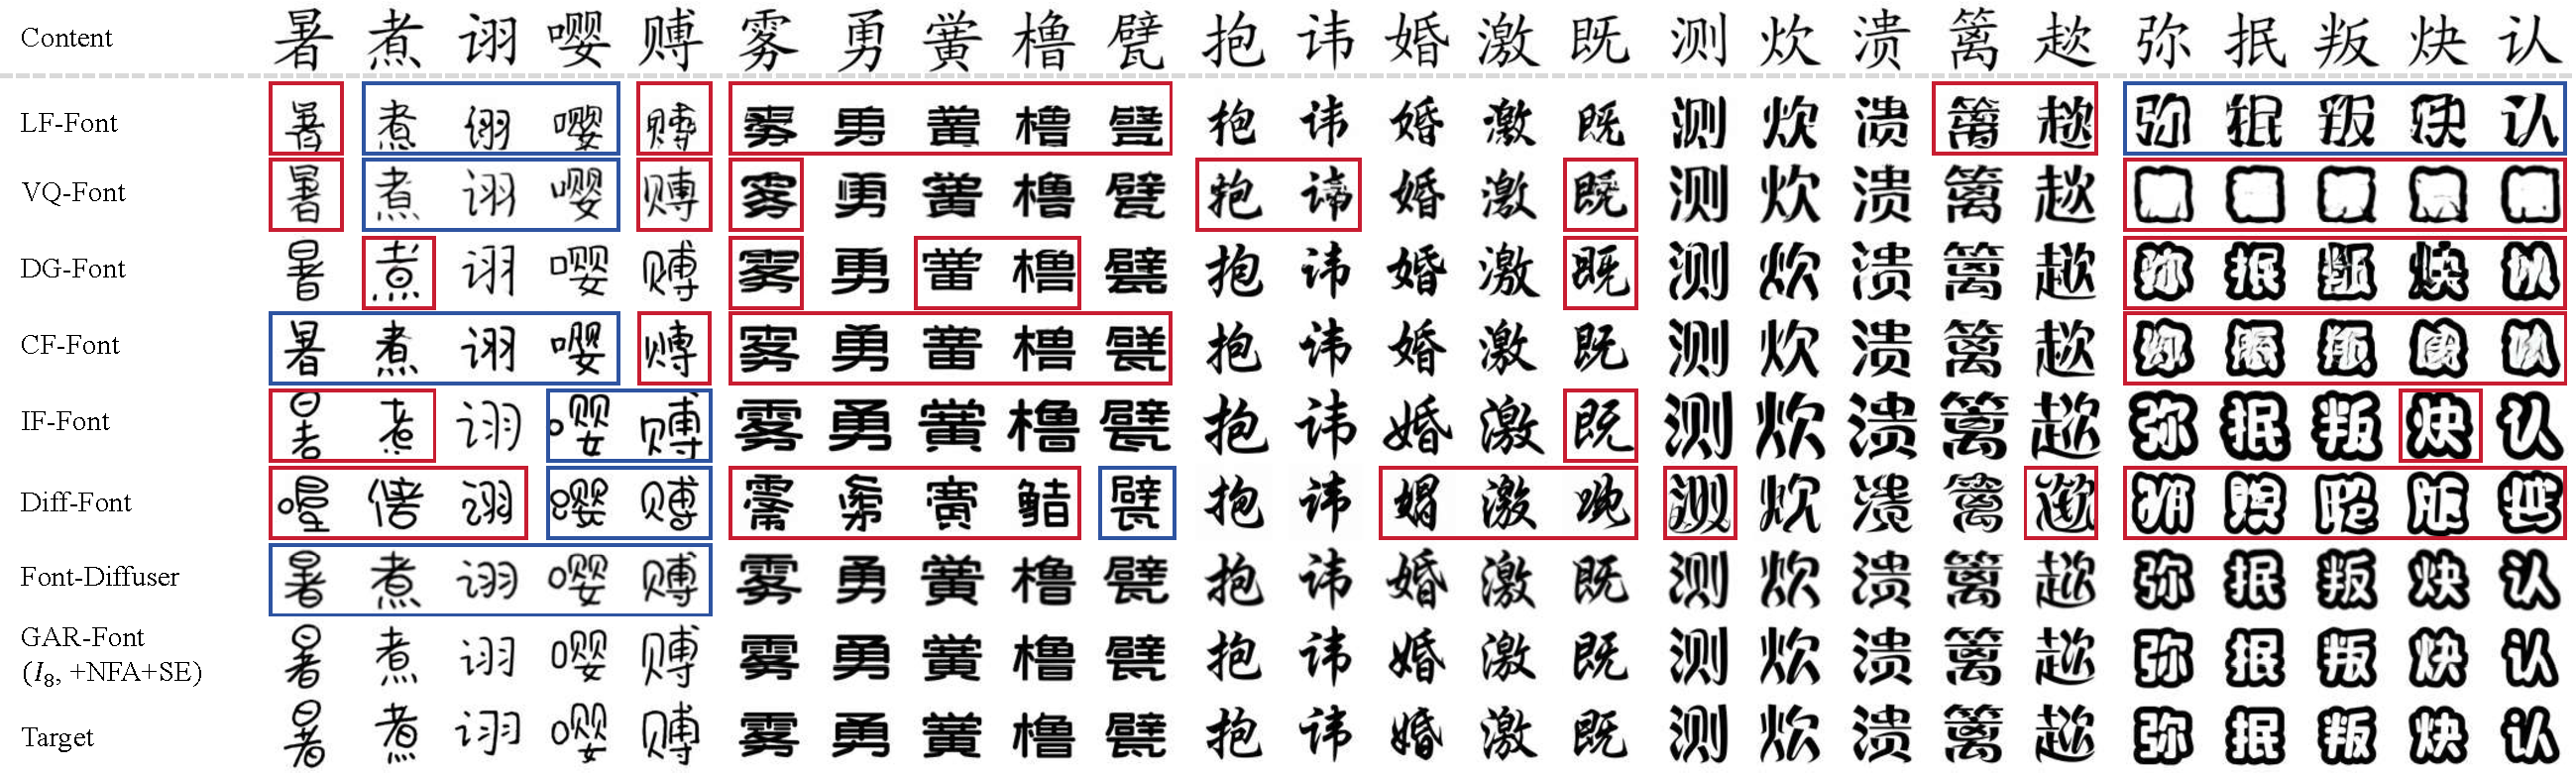
\includegraphics[width=\linewidth]{SUPP_IMGS/EX_Visualization/table_Main1_UFSC_Large.pdf}
        \vspace{-3mm}
        \caption{\textit{UFSC}, Large dataset}
        \vspace{1mm}
        \label{fig: supple_main1_ufsc_large}
    \end{subfigure}

    \begin{subfigure}{0.91\linewidth}
        \centering
        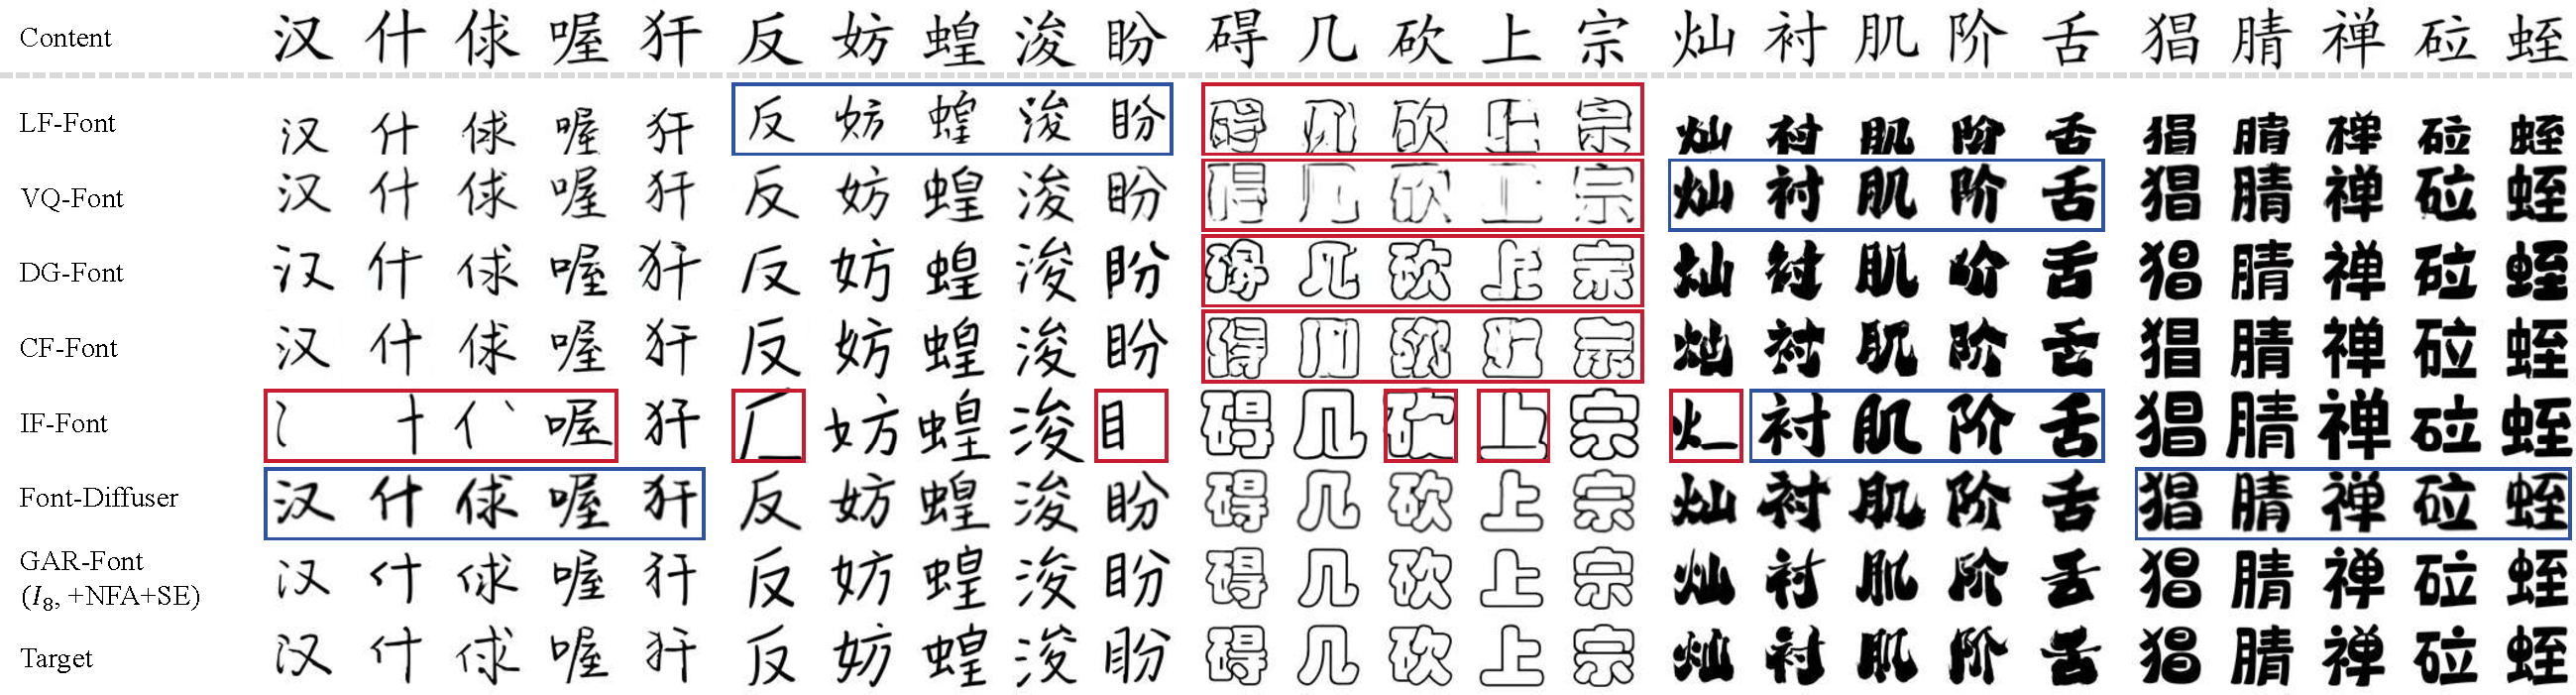
\includegraphics[width=\linewidth]{SUPP_IMGS/EX_Visualization/table_Main1_UFUC_Large.pdf}
        \vspace{-3mm}
        \caption{\textit{UFUC}, Large dataset}
        \vspace{1mm}
        \label{fig: supple_main1_ufuc_large}
    \end{subfigure}
    \vspace{-2mm}
    \caption{
        Qualitative results on vision-only FFG across \textit{UFSC/UFUC} protocols and Small/Large datasets.
        \textcolor{ex1figure_red}{\fbox{\rule{0pt}{4pt}\rule{4pt}{0pt}}} /
        \textcolor{ex1figure_blue}{\fbox{\rule{0pt}{4pt}\rule{4pt}{0pt}}}
        indicate structural errors and style mismatches.
    }
    
    \vspace{-4mm}
    \label{fig: supple_main1_all}
\end{figure*}


\subsection{On Multimodal Style Encoder's Adaptation}
% UFSC,  UFUC,  Large dataset
We compare our decoupled multimodal training paradigm against joint training of the multimodal style encoder. While quantitative results are provided in Section 5.3, we present the full set of qualitative comparisons here.

Figure ~\ref{fig: supple_abl4_all} presents visual comparisons on (\textit{UFSC}, Large) and (\textit{UFUC}, Large). The results reveal that GAR-Font($M_2$/$M_4$), trained with the decoupled training scheme, generate glyphs whose font styles more closely align with the target compared to the jointly trained GAR-Font($VL_2$/$VL_4$). They also demonstrate better character-structure accuracy. The decoupled training strategy enables the model to fully leverage the visual encoder’s representational capacity, thereby preserving fine-grained style features and structural priors that may be harder to retain under joint optimization.


\begin{figure*}[tp] % [p] 强制单独一页
    \centering

    % =========================================
    % 第一组：Pre-Train
    % =========================================
    
    % -------- (a) Pre --------
    \begin{subfigure}{0.92\linewidth} % 建议缩小到 0.9 或 0.85 以防超高
        \centering
        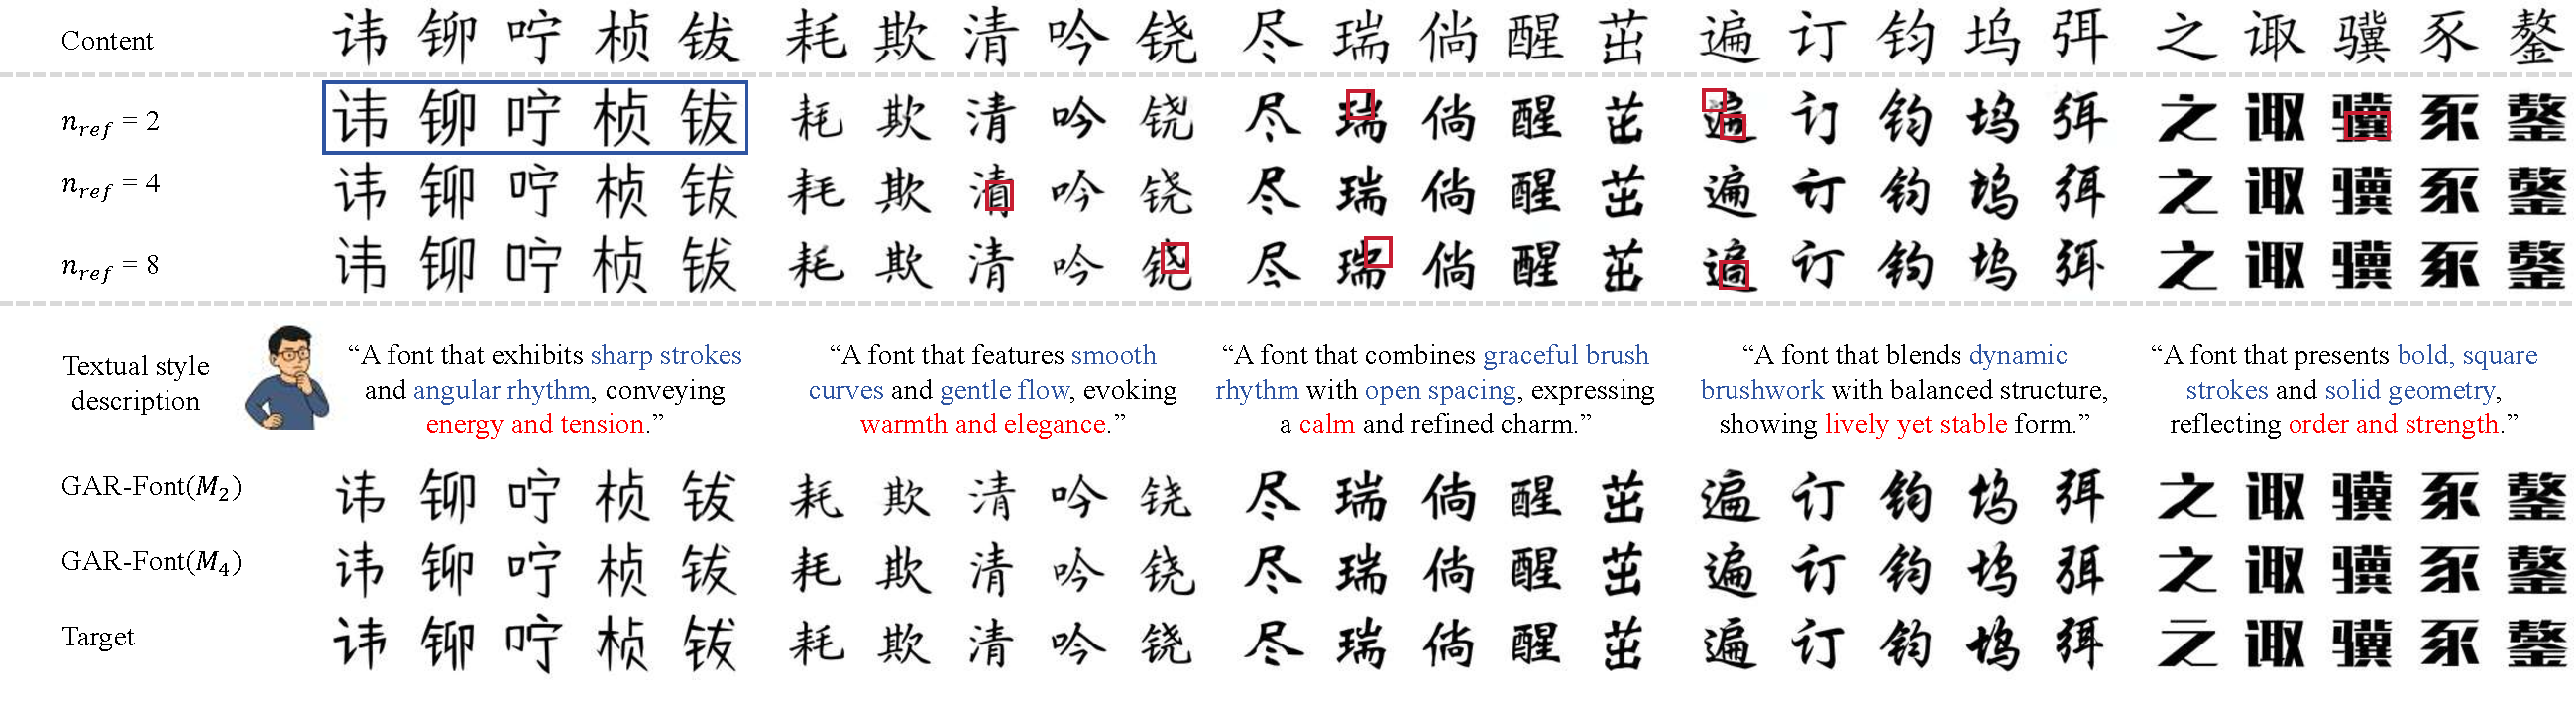
\includegraphics[width=\linewidth]{SUPP_IMGS/EX_Visualization/table2_supple_UFSC_Large_Pre.pdf}
        \caption{\textit{UFSC}, Large dataset}
        \label{fig: supple_main2_ufsc_large_pre}
    \end{subfigure}
    \\ % 强制换行
    \vspace{1mm} % 稍微减少间距
    % -------- (b) Pre --------
    \begin{subfigure}{0.92\linewidth}
        \centering
        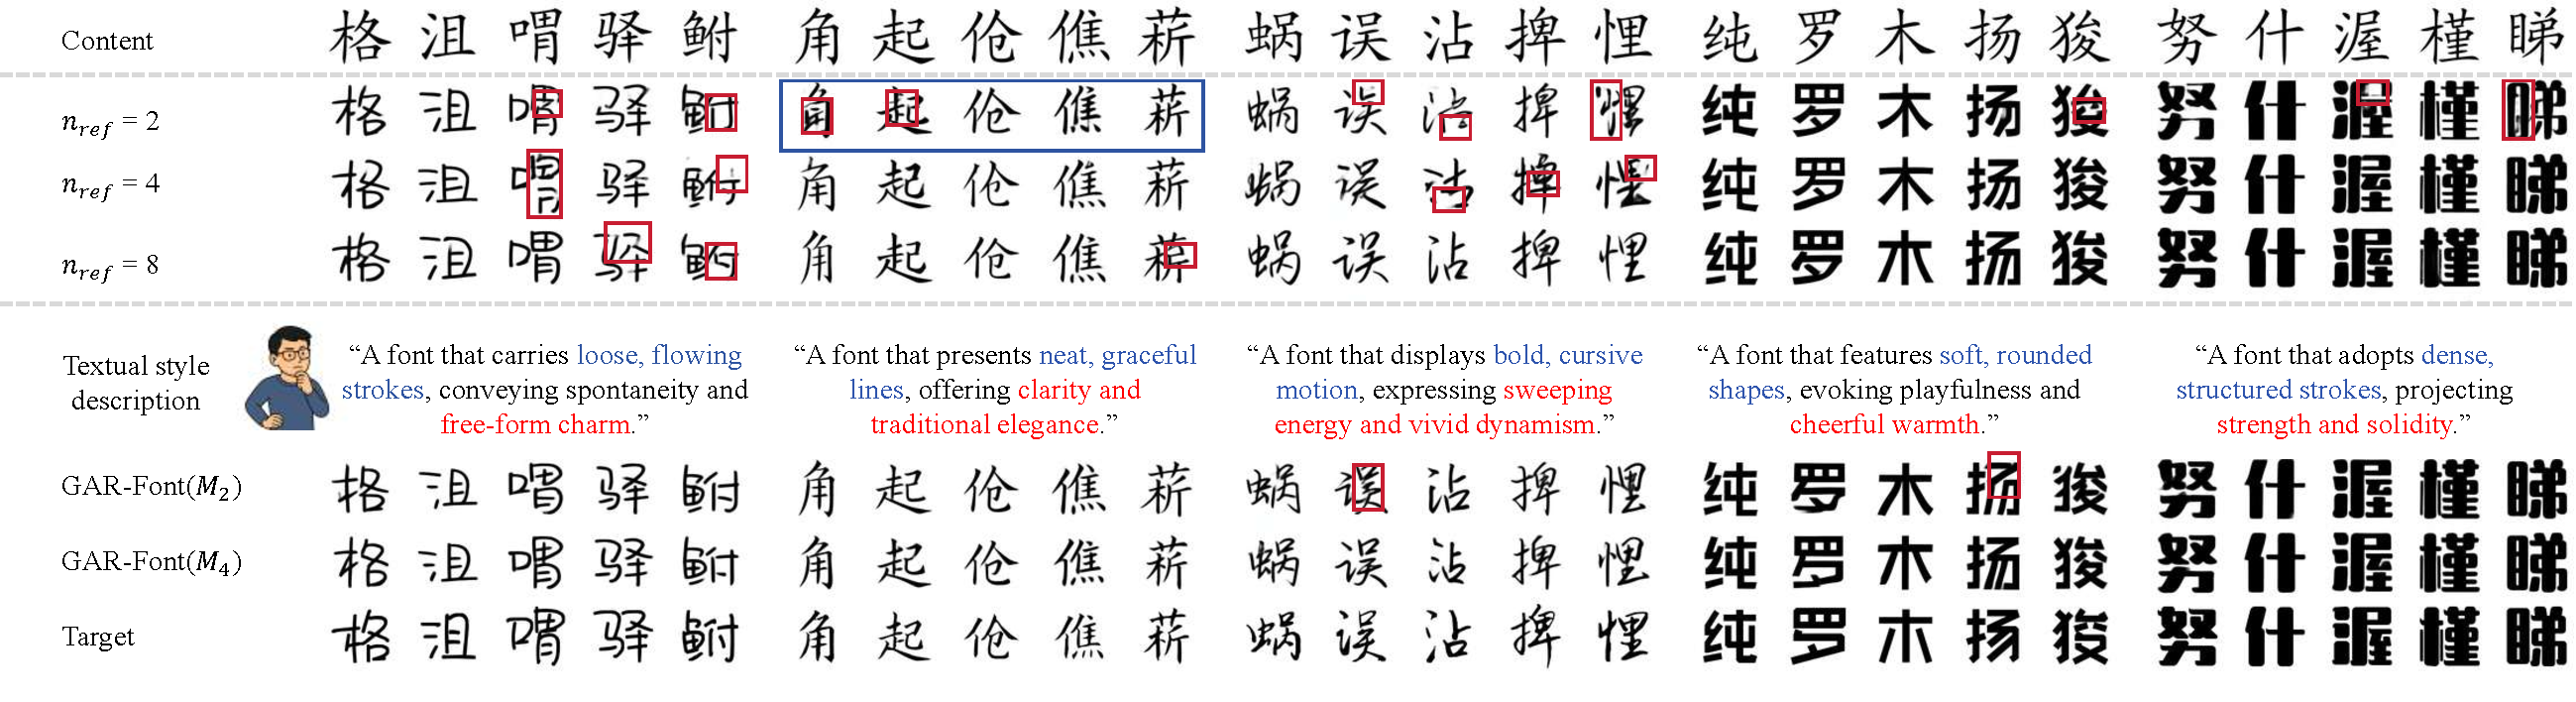
\includegraphics[width=\linewidth]{SUPP_IMGS/EX_Visualization/table2_supple_UFUC_Large_Pre.pdf}
        \caption{\textit{UFUC}, Large dataset}
        \label{fig: supple_main2_ufuc_large_pre}
    \end{subfigure}
    \vspace{-2mm}
    
    % -------- 第一组 Caption --------
    \caption{
        Qualitative results of Pre-Train multimodal FFG under \textit{UFSC} and \textit{UFUC} protocols
        (Large dataset). 
        \textcolor{ex2figure_red}{\fbox{\rule{0pt}{4pt}\rule{4pt}{0pt}}} denotes local slight structural mistakes, 
        and \textcolor{ex2figure_blue}{\fbox{\rule{0pt}{4pt}\rule{4pt}{0pt}}} marks stylistic drift.
    }
    \label{fig: supple_main2_large_pre_all}

    \vspace{1em} % 在两个大图组之间增加明显间距

    % =========================================
    % 第二组：Post-Refine
    % =========================================

    % -------- (a) Post --------
    \begin{subfigure}{0.92\linewidth}
        \centering
        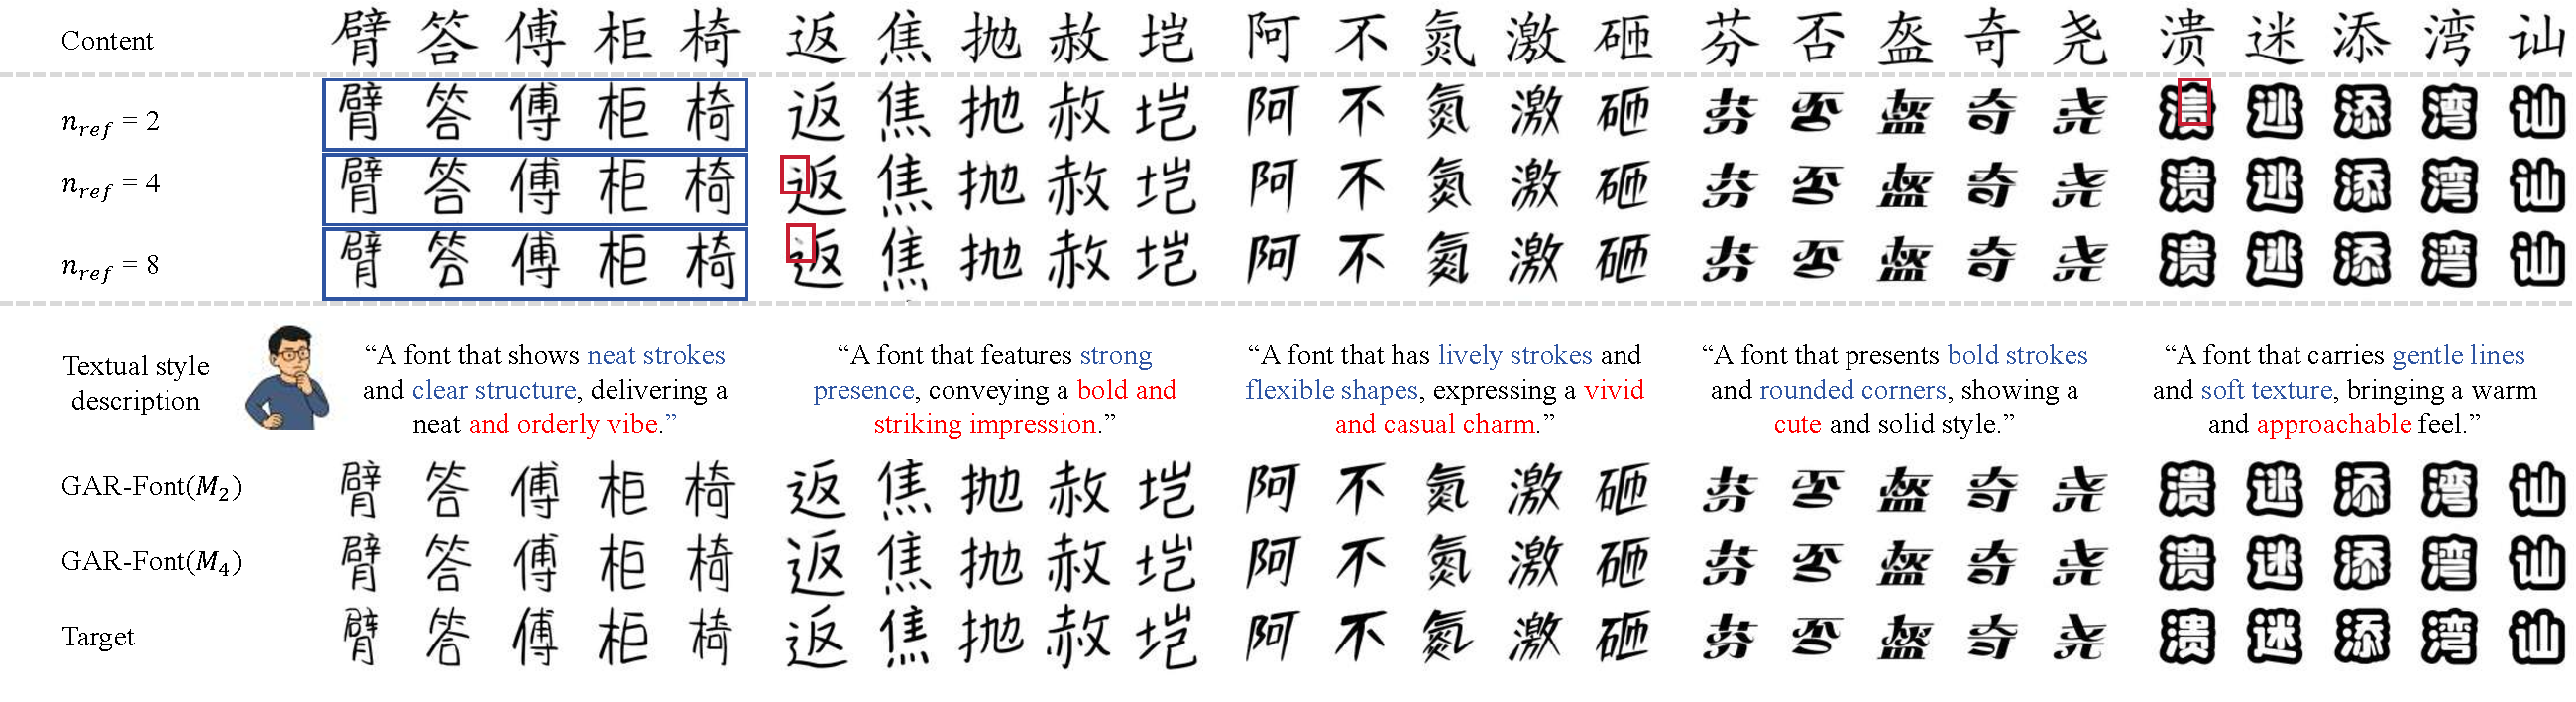
\includegraphics[width=\linewidth]{SUPP_IMGS/EX_Visualization/table2_supple_UFSC_Large_Post.pdf}
        \caption{\textit{UFSC}, Large dataset}
        \label{fig: supple_main2_ufsc_large_post}
    \end{subfigure}
    \\ % 强制换行
    \vspace{1mm}
    % -------- (b) Post --------
    \begin{subfigure}{0.92\linewidth}
        \centering
        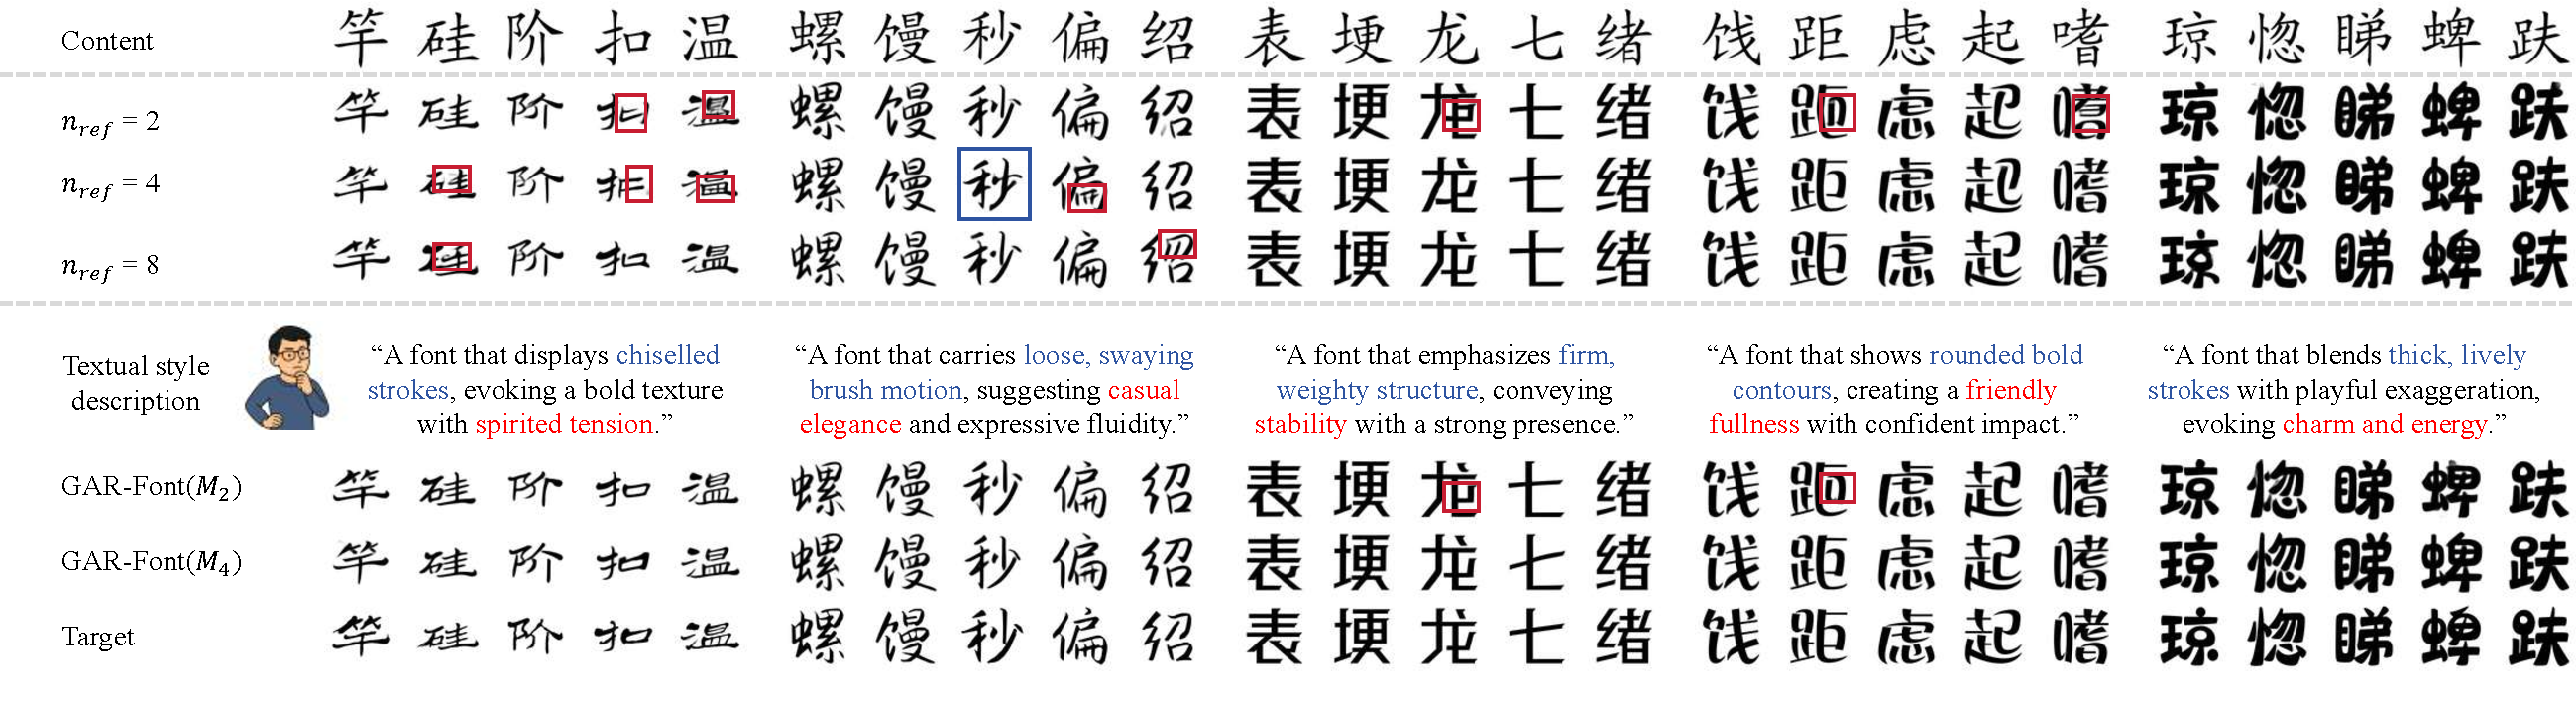
\includegraphics[width=\linewidth]{SUPP_IMGS/EX_Visualization/table2_supple_UFUC_Large_Post.pdf}
        \caption{\textit{UFUC}, Large dataset}
        \label{fig: supple_main2_ufuc_large_post}
    \end{subfigure}
    \vspace{-2mm}

    % -------- 第二组 Caption --------
    \caption{
        Qualitative results of Post-Refine multimodal FFG under \textit{UFSC} and \textit{UFUC} protocols
        (Large dataset). 
        \textcolor{ex2figure_red}{\fbox{\rule{0pt}{4pt}\rule{4pt}{0pt}}} denotes local slight structural mistakes, 
        and \textcolor{ex2figure_blue}{\fbox{\rule{0pt}{4pt}\rule{4pt}{0pt}}} marks stylistic drift.
    }
    \label{fig: supple_main2_large_post}

\end{figure*}




% \begin{figure*}[t]
%     \centering

%     % -------- (a) --------
%     \begin{subfigure}{0.95\linewidth}
%         \centering
%         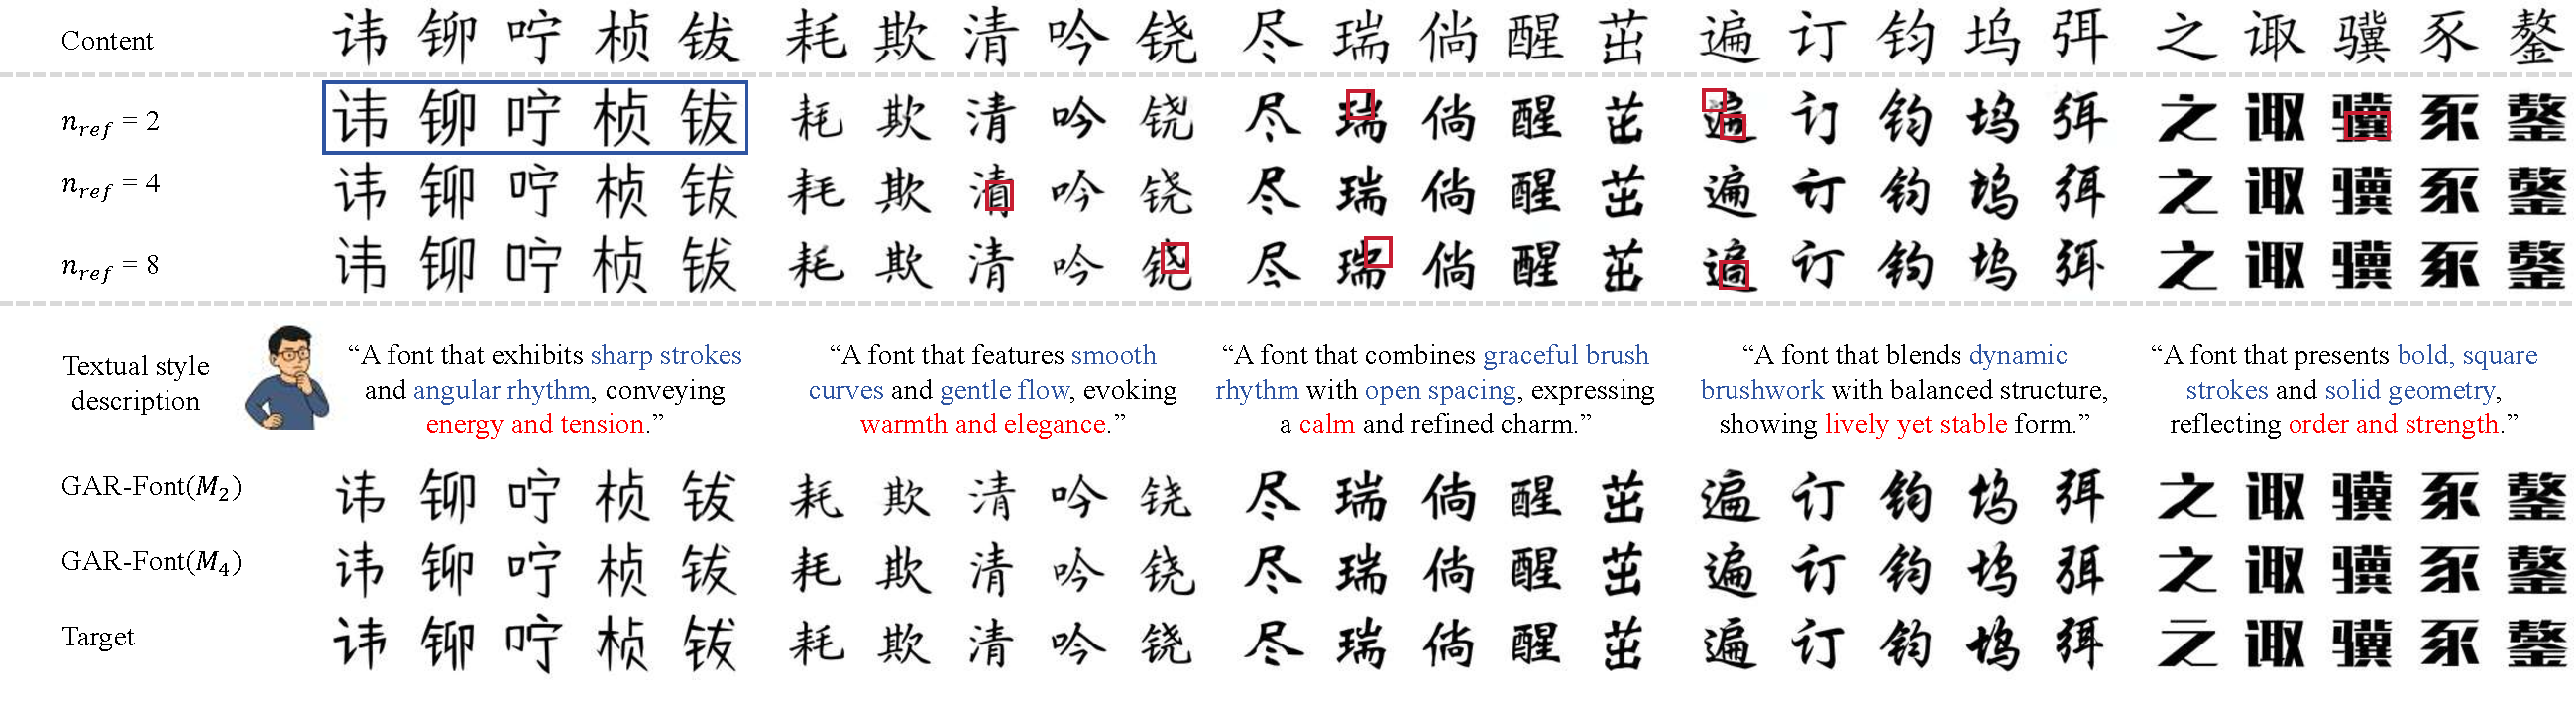
\includegraphics[width=\linewidth]{SUPP_IMGS/EX_Visualization/table2_supple_UFSC_Large_Pre.pdf}
%         \caption{UFSC, \textit{Large} dataset}
%         \label{fig: supple_main2_ufsc_large_pre}
%     \end{subfigure}

%     \vspace{2mm}

%     % -------- (b) --------
%     \begin{subfigure}{0.95\linewidth}
%         \centering
%         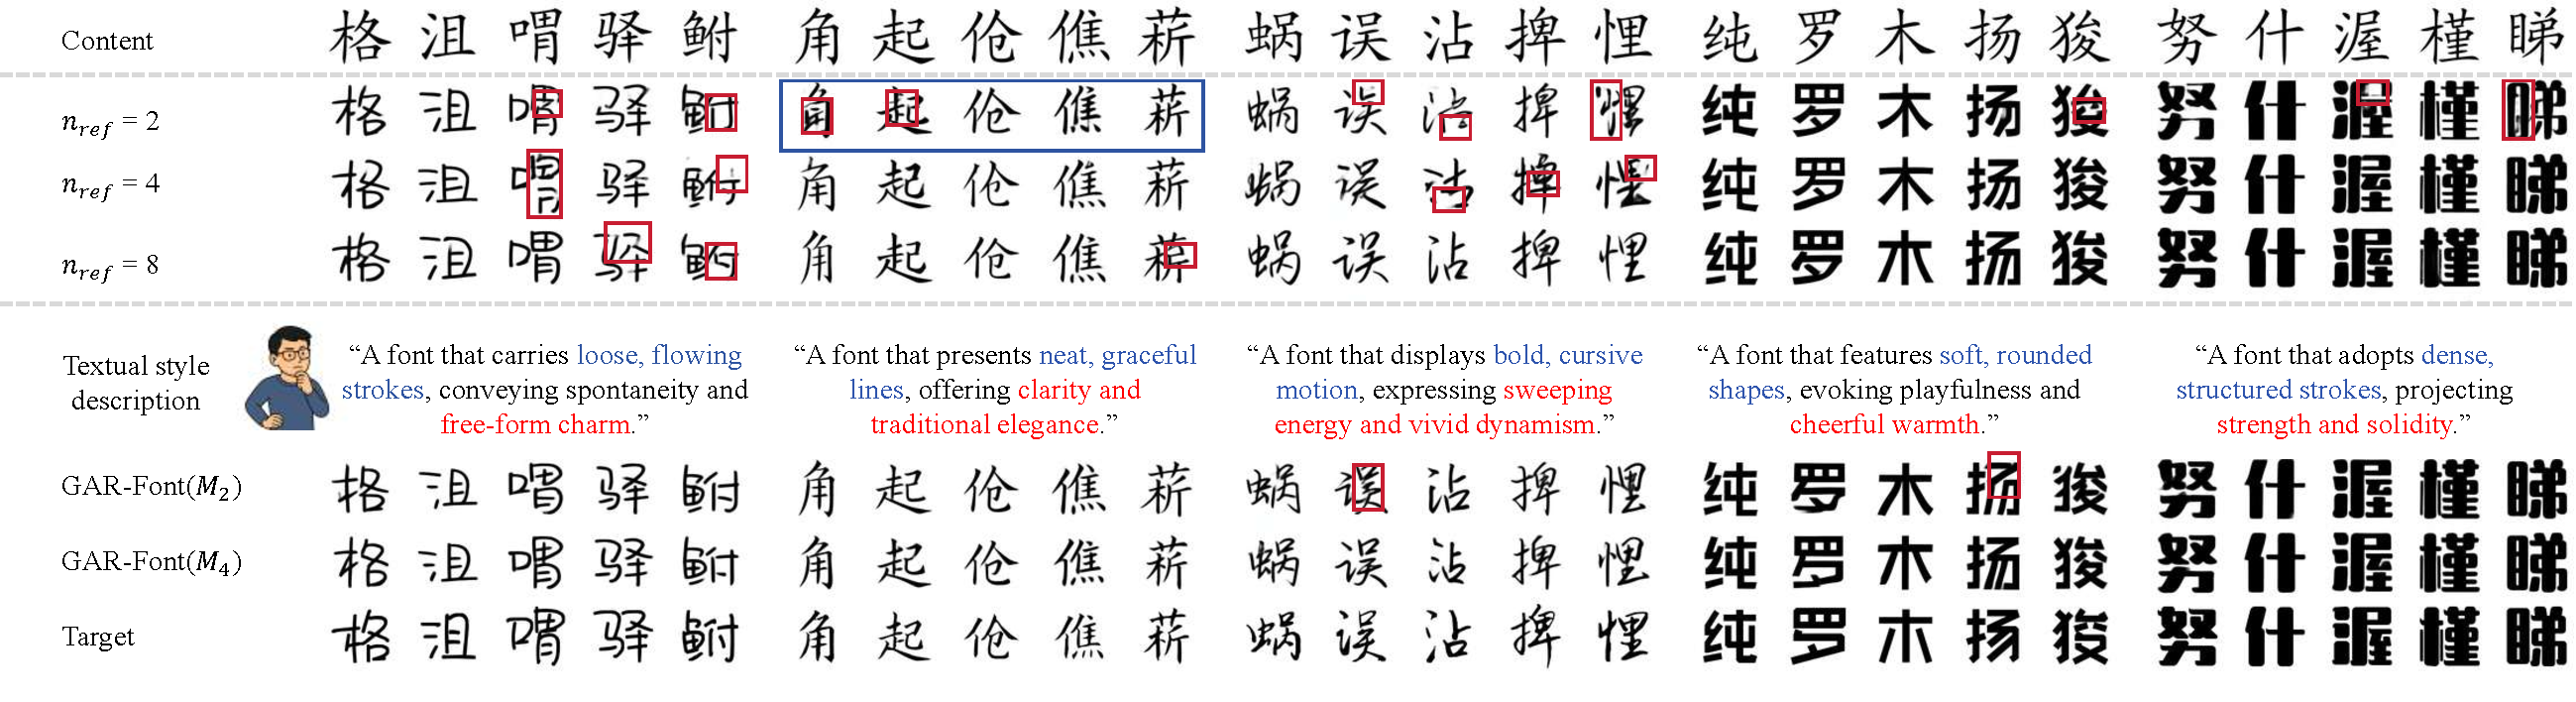
\includegraphics[width=\linewidth]{SUPP_IMGS/EX_Visualization/table2_supple_UFUC_Large_Pre.pdf}
%         \caption{UFUC, \textit{Large} dataset}
%         \label{fig: supple_main2_ufuc_large_pre}
%     \end{subfigure}

%     \vspace{2mm}

%     % -------- main caption --------
%     \caption{
%         Qualitative results on Pre-Train multimodal FFG under UFSC and UFUC protocols
%         (\textit{Large} dataset). 
%         \textcolor{ex2figure_red}{\fbox{\rule{0pt}{4pt}\rule{4pt}{0pt}}} denotes local slight structural mistakes,
%         and \textcolor{ex2figure_blue}{\fbox{\rule{0pt}{4pt}\rule{4pt}{0pt}}} marks samples with stylistic drift.
%     }
%     \label{fig: supple_main2_large_pre_all}
% \end{figure*}



% \begin{figure*}[t]
%     \centering

%     % -------- (a) --------
%     \begin{subfigure}{0.95\linewidth}
%         \centering
%         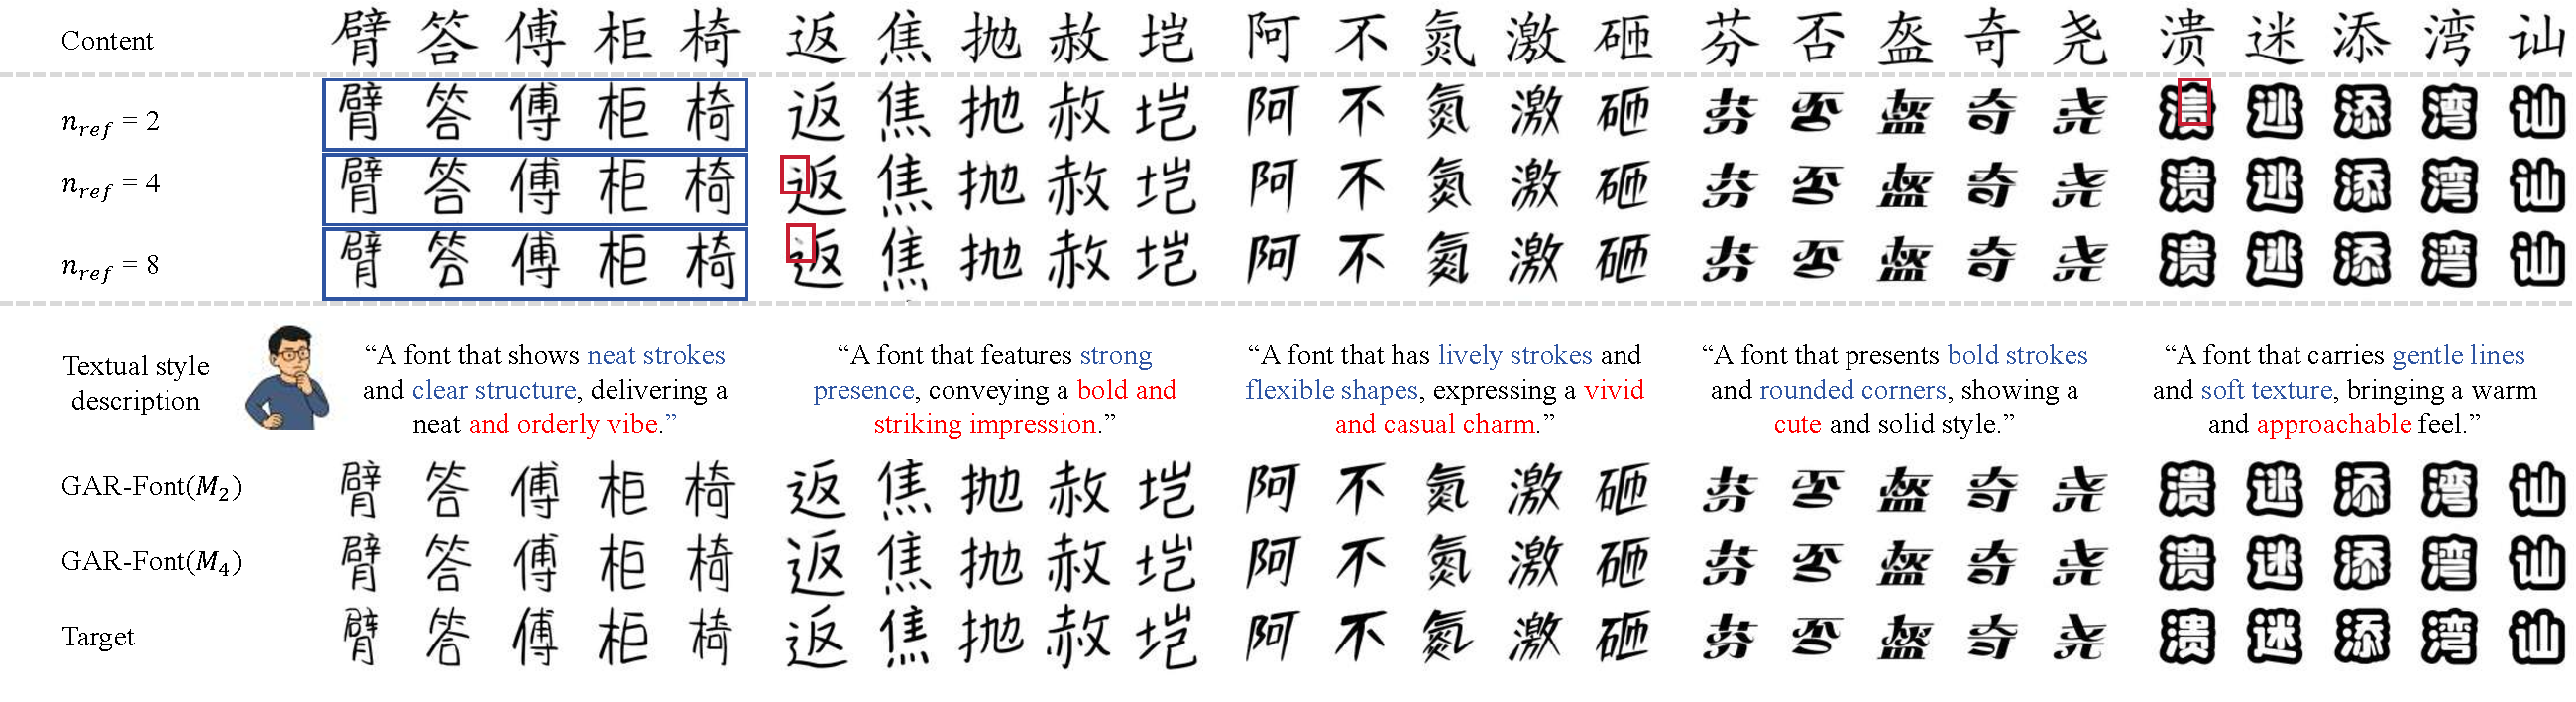
\includegraphics[width=\linewidth]{SUPP_IMGS/EX_Visualization/table2_supple_UFSC_Large_Post.pdf}
%         \caption{UFSC, \textit{Large} dataset}
%         \label{fig: supple_main2_ufsc_large_post}
%     \end{subfigure}

%     \vspace{2mm}

%     % -------- (b) --------
%     \begin{subfigure}{0.95\linewidth}
%         \centering
%         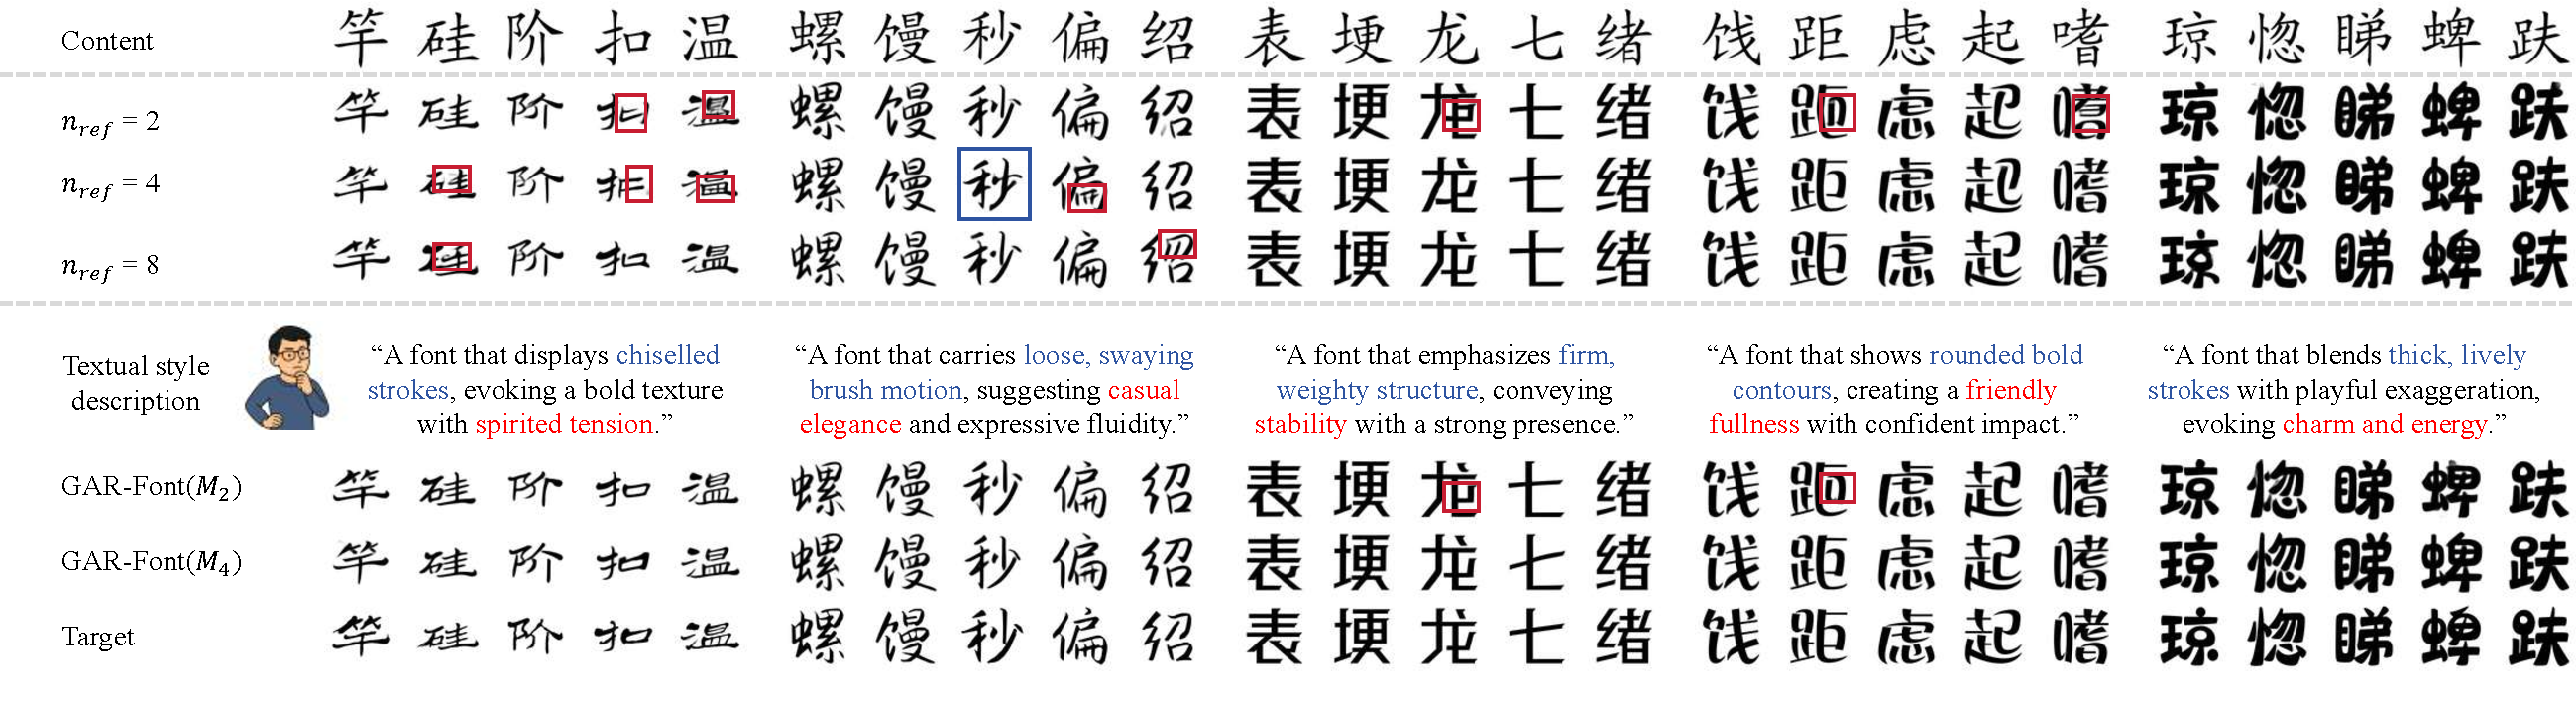
\includegraphics[width=\linewidth]{SUPP_IMGS/EX_Visualization/table2_supple_UFUC_Large_Post.pdf}
%         \caption{UFUC, \textit{Large} dataset}
%         \label{fig: supple_main2_ufuc_large_post}
%     \end{subfigure}

%     \vspace{2mm}

%     % -------- main caption --------
%     \caption{
%         Qualitative results of Post-Refine multimodal FFG under UFSC and UFUC protocols
%         (\textit{Large} dataset). 
%         \textcolor{ex2figure_red}{\fbox{\rule{0pt}{4pt}\rule{4pt}{0pt}}} denotes local slight structural mistakes, 
%         and \textcolor{ex2figure_blue}{\fbox{\rule{0pt}{4pt}\rule{4pt}{0pt}}} marks stylistic drift.
%     }
%     \label{fig: supple_main2_large_post}
% \end{figure*}
\begin{figure*}[t]
  \centering
  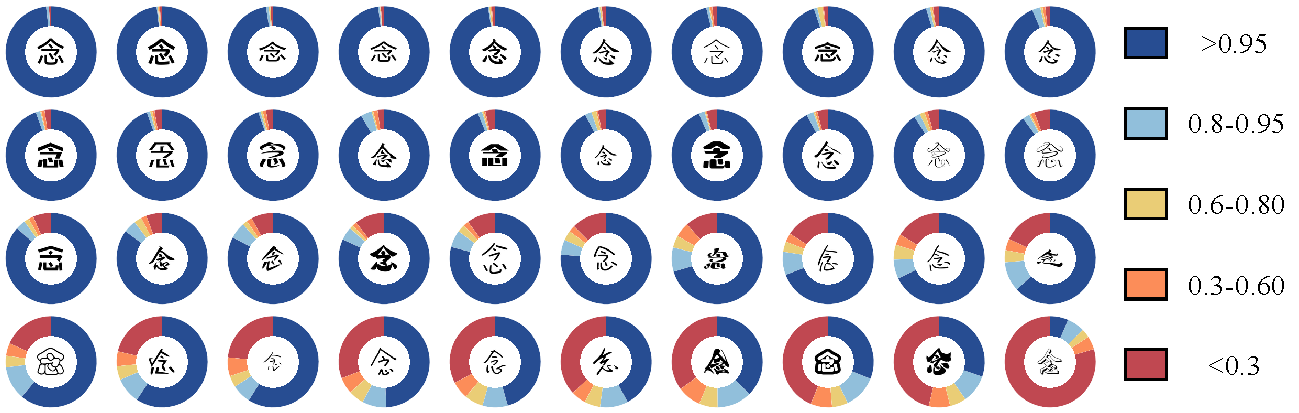
\includegraphics[width=0.95\linewidth]{SUPP_IMGS/Failure_Analysis/analysis_final.pdf}
  \vspace{-3mm}
  \caption{Content confidence distribution of GAR-Font generated characters across different font styles. Each pie chart corresponds to a specific font, indicated by the central character. The color segments represent the proportion of samples falling into different content confidence ranges, highlighting that more complex styles tend to have lower content confidence.}
  \vspace{-3mm}
  \label{fig:supple_analysis}
\end{figure*}



\begin{figure}[t]
  \centering
  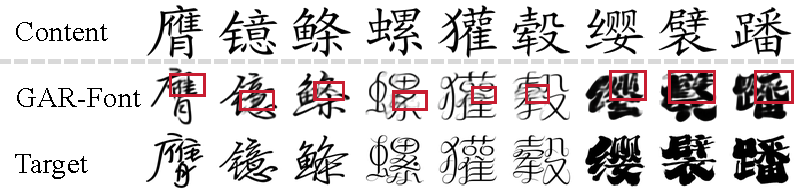
\includegraphics[width=0.95\linewidth]{SUPP_IMGS/Failure_Analysis/Failure_revised.pdf}
  \vspace{-3mm}
  \caption{Failure cases. \textcolor{ex2figure_red}{\fbox{\rule{0pt}{4pt}\rule{4pt}{0pt}}} highlights regions with dense details where GAR-Font tends to produce distorted strokes.}
  \vspace{-3mm}
  \label{fig:supple_failure_cases}
\end{figure}

\section{Visualization Results}
\label{sec:vis_results}
\subsection{Comparison on Few-shot Font Generation}
% UFSC， UFUC，  Large dataset
% UFSC,  UFUC,  Small dataset
We provide complete visualizations for the experiment in Section 5.1. In addition to the main results, Figure~\ref{fig: supple_main1_all} offer a granular analysis of our architectural decisions. 

In Figure~\ref{fig: supple_main1_all}, we show the full qualitative comparisons of visual-only FFG models trained on Small and Large datasets, evaluated under both \textit{UFSC} and \textit{UFUC} protocols. These results indicate that methods such as LF--Font, VQ-Font, DG-Font, CF-Font and Diff-Font often fail to preserve structural fidelity in intricate fonts. IF-Font tends to produce incomplete characters, while Font-Diffuser generates with inaccurate stroke widths. In contrast, GAR-Font($I_8$,+NFA+SE) achieves the best style fidelity while maintaining structural consistency, effectively capturing fine stroke details of the target fonts.


\subsection{Efficient Vision-Language Adaptation}

\subsubsection{Pretrain}
% UFSC， UFUC，  Large dataset

We provide full qualitative results complementing the experiment in Section~5.2. 
In Figure~\ref{fig: supple_main2_large_pre_all}, we show multimodal FFG comparisons under both \textit{UFSC} and \textit{UFUC} settings on the Large dataset, illustrating the improvements introduced by incorporating textual style descriptions in GAR-Font($M_2$) and GAR-Font($M_4$) compared with their vision-only counterparts. With textual style guidance, GAR-Font($M_2$) and GAR-Font($M_4$) better align with the target style, generating glyphs with strokes closely matching the target and improved structural fidelity.


\subsubsection{Post-Refinement}
% UFSC， UFUC，  Large dataset
To further assess the potential of our efficient vision–language adaptation, we apply the complete post-refinement pipeline (NFA and SE) to GAR-Font($M_2$) and GAR-Font($M_4$). 
Figure~\ref{fig: supple_main2_ufsc_large_post} presents qualitative results under \textit{UFSC} and \textit{UFUC} on the Large dataset. Applying NFA and SE post-refinement significantly improves both structural and style fidelity for all models. Textual guidance further enables GAR-Font($M_2$) and GAR-Font($M_4$) to more accurately capture the target style, yielding glyphs with improved style fidelity.

\subsection{More GAR-Font Generation Examples}
To illustrate the capabilities of GAR-Font, we generate the full GB2312 character set for five test fonts with GAR-Font($I_8$, +NFA+SE, trained on Large dataset) and randomly select 1,280 samples from each font. The generated glyphs are shown in Figures ~\ref{fig: add_sheet_1}-~\ref{fig: add_sheet_5} , demonstrating the model’s ability to produce large-scale character sets while faithfully preserving each font’s distinctive stylistic features.


\section{Failure Cases and Analysis}
\label{sec:Failure_cases}

While GAR-Font generally performs well, distortions and blurring occasionally appear in dense-stroke regions of highly complex fonts (\cref{fig:supple_failure_cases}). To investigate this, we applied a content classifier to all \textit{UFUC} samples generated by GAR-Font($I_8$,+NFA+SE), using the softmax output as a measure of content confidence. The results reveal a clear trend: content confidence notably decreases as stylistic complexity increases (\cref{fig:supple_analysis}), suggesting the model sometimes sacrifices structural accuracy to better capture stylistic features.

We hypothesize that this structural degradation results from the error accumulation inherent in autoregressive modeling. Without explicit structural constraints, the model tends to drift when generating intricate stroke patterns. A promising direction for future work is to incorporate explicit structural priors, such as character skeletons or stroke sequences, to guide the generation process. This would help preserve structural fidelity in complex styles.


\begin{figure*}
    \centering
    \includegraphics[width=0.95\linewidth]{SUPP_IMGS/Samples_Sheet/gen_soft_BigruixianBoldkGBV1.0_sample_12.png}
    \vspace{-3mm}
    \caption{Generated glyphs from test fonts using GAR-Font($I_8$, +NFA+SE, Large dataset).}
    \label{fig: add_sheet_1}
    \vspace{-3mm}
\end{figure*}
\clearpage
\begin{figure*}
    \centering
    \includegraphics[width=0.95\linewidth]{SUPP_IMGS/Samples_Sheet/gen_soft_FZBaiZhouRenZheTiS_sample_13.png}
    \vspace{-3mm}
    \caption{Generated glyphs from test fonts using GAR-Font($I_8$, +NFA+SE, Large dataset).}
    \label{fig: add_sheet_2}
    \vspace{-3mm}
\end{figure*}
\clearpage
\begin{figure*}
    \centering
    \includegraphics[width=0.95\linewidth]{SUPP_IMGS/Samples_Sheet/gen_soft_FZSJ-MINGYSJZ_sample_14.png}
    \vspace{-3mm}
    \caption{Generated glyphs from test fonts using GAR-Font($I_8$, +NFA+SE, Large dataset).}
    \label{fig: add_sheet_3}
    \vspace{-3mm}
\end{figure*}
\clearpage
\begin{figure*}
    \centering
    \includegraphics[width=0.95\linewidth]{SUPP_IMGS/Samples_Sheet/gen_soft_MiNiJianYouXian_sample_9.png}
    \vspace{-3mm}
    \caption{Generated glyphs from test fonts using GAR-Font($I_8$, +NFA+SE, Large dataset).}
    \label{fig: add_sheet_4}
    \vspace{-3mm}
\end{figure*}
\clearpage
\begin{figure*}
    \centering
    \includegraphics[width=0.95\linewidth]{SUPP_IMGS/Samples_Sheet/gen_soft_zihun40hao-xiaochengfeifanti-Regular_sample_9.png}
    \vspace{-3mm}
    \caption{Generated glyphs from test fonts using GAR-Font($I_8$, +NFA+SE, Large dataset).}
    \label{fig: add_sheet_5}
    \vspace{-3mm}
\end{figure*}
\clearpage